\documentclass[11pt,letterpaper]{article}
\usepackage[utf8]{inputenc}
\usepackage{amsmath}
\usepackage{amsfonts}
\usepackage{amssymb}
\usepackage{graphicx}
\usepackage{booktabs}
\usepackage{natbib}
\usepackage{hyperref}
\usepackage{array}
\usepackage{longtable}
\usepackage{xfp}
\usepackage{siunitx}
\usepackage{newunicodechar}
\usepackage{adjustbox}
\usepackage{subcaption}
\usepackage{tcolorbox}
\usepackage{pdfpages}
\usepackage{afterpage}
\usepackage{float}
\newunicodechar{∞}{\ensuremath{\infty}}

% Data placeholders - UPDATED with actual values from analysis
\newcommand{\totalConversations}{229}
\newcommand{\numEmbeddingModels}{5}

% Core findings from actual data
\newcommand{\meanInvarianceScore}{0.377}
\newcommand{\medianInvarianceScore}{0.547}

% Distance matrix correlations from heatmaps
\newcommand{\distanceMatrixCorrelation}{0.879}
\newcommand{\distanceCorrRange}{(0.521, 0.957)}
\newcommand{\minPairwiseCorr}{0.521}
\newcommand{\maxPairwiseCorr}{0.957}

% Model-specific correlations from data
\newcommand{\transformerInternalCorr}{0.827}
\newcommand{\classicalInternalCorr}{0.934}
\newcommand{\crossParadigmCorr}{0.616}

% Specific model pair correlations from heatmap
\newcommand{\miniLMmpnetCorr}{0.855}
\newcommand{\miniLMwordTovecCorr}{0.659}
\newcommand{\wordTovecGloveCorr}{0.931}

% Visual pattern metrics
\newcommand{\blockPatternConsistency}{high}
\newcommand{\trajectoryShapeAgreement}{moderate}
\newcommand{\densityPeakAlignment}{variable}

% Phase detection performance - HIGHLY VARIABLE
\newcommand{\phaseDetectionF}{0.16}
\newcommand{\phaseAgreementRange}{(-0.14, 0.76)}
\newcommand{\phaseDetectionBest}{0.76}
\newcommand{\phaseDetectionWorst}{-0.14}
\newcommand{\phaseDetectionFRange}{(0.08, 0.36)}

% Statistical validation
\newcommand{\bootstrapIterations}{10000}
\newcommand{\nullModelPValue}{0.001}
\newcommand{\nullBaselineCorr}{0.082}

% Hypothesis test results
\newcommand{\tiersPassed}{3/3}
\newcommand{\meanEffectSize}{0.152}
\newcommand{\hOnepvalue}{2.8606e-08}
\newcommand{\hTwopvalue}{1.4507e-10}

% Conversation metrics
\newcommand{\minConvLength}{118}
\newcommand{\maxConvLength}{235}
\newcommand{\meanConvLength}{183.2}

% Figure paths
\newcommand{\figuresPath}{../analysis/analysis_output/figures/}

\title{The Geometry of Conversation: Evidence for High-Dimensional Semantic Space from Multi-Model Invariance}

\author{
Marco R. Garcia \\
marco@erulabs.ai
}

\date{\today}

\begin{document}

\maketitle

\begin{abstract}
We present empirical evidence that conversations exhibit consistent geometric signatures when projected into different embedding spaces, alongside surprising variability in local feature detection. Analyzing \totalConversations{} multi-agent AI dialogues from our prior study on social dynamics \citep{garcia2025peer}, we examine whether geometric properties of conversational trajectories remain consistent across \numEmbeddingModels{} fundamentally different embedding models. Our analysis reveals a striking dichotomy: while global geometric patterns (distance matrices, trajectory shapes) show remarkable consistency across both transformer-based and classical embeddings (correlations ranging from \minPairwiseCorr{} to \maxPairwiseCorr{}), local phase detection exhibits extreme variability (F1 scores from 0.08 to 0.36, agreement correlations from -0.14 to 0.76). This pattern—high global consistency with low local agreement—suggests that different embedding models may capture distinct projections of conversations existing in a higher-dimensional semantic space. Transport-based analysis confirms this interpretation, showing threefold increases in cross-paradigm distances compared to within-paradigm distances. These findings establish that while geometric analysis of conversation captures genuine structural properties, the global-local dichotomy implies fundamental limits on fine-grained analysis and raises intriguing questions about the true dimensionality of conversational dynamics.
\end{abstract}

\section{Introduction}

In our recent investigation of AI social dynamics \citep{garcia2025peer}, we documented unexpected peer pressure effects in multi-agent conversations. These behavioral phenomena (breakdown cascades, recovery mechanisms, behavioral territories) revealed complex dynamics that traditional analysis methods struggled to explain. Specifically, we observed that 79.1\% of full reasoning model conversations exhibited peer pressure effects, with 55.2\% cascading to breakdown states characterized by mystical language and symbolic responses. This observation motivated an exploratory question: might conversations have underlying mathematical structure that could provide new perspectives on these dynamics?

The present work investigates whether these behavioral dynamics have consistent geometric correlates across embedding spaces, potentially enabling prediction and intervention. By \textit{geometric signatures}, we mean measurable properties like pairwise distance matrices between messages, trajectory shapes as conversations evolve, and density patterns in the embedding space. By \textit{conversational trajectories}, we mean the path traced through embedding space as a conversation progresses from message to message.

To understand our approach, consider how a three-dimensional sculpture casts different two-dimensional shadows depending on the viewing angle. The shadows agree on basic properties (the object has extent, connected regions) but differ in details (precise boundaries, local features). Similarly, different embedding models might capture different "views" of conversations existing in a higher-dimensional space.

We test for geometric invariance using \totalConversations{} multi-agent dialogues from our social dynamics study. By examining conversational trajectories through \numEmbeddingModels{} diverse embedding models (including both transformer and classical approaches), we can assess whether observed patterns reflect genuine conversational structure or merely artifacts of specific architectures.

Our key empirical findings reveal an unexpected dichotomy:
\begin{enumerate}
\item \textbf{Global geometry is remarkably consistent}: Distance matrices and trajectory shapes show strong correlations across all embedding models
\item \textbf{Local features are surprisingly variable}: Phase detection and fine-grained structure show poor cross-model agreement
\item \textbf{This pattern persists across paradigms}: Even fundamentally different approaches agree on macro-structure while disagreeing on micro-structure
\end{enumerate}

\section{Background and Related Work}

\subsection{The Geometric Turn in Language Understanding}

Recent advances in NLP have revealed that language models encode rich geometric structure. \citet{reif2019visualizing} demonstrated that BERT segregates semantic and syntactic information into distinct subspaces, establishing that transformer embeddings have interpretable geometric organization. This finding motivates our question: if individual models exhibit geometric structure, do different models capture the same structure?

\citet{ethayarajh2019contextual} complicated this picture by showing that contextual embeddings occupy narrow cones in vector space, challenging assumptions about isotropy. Their work is crucial for our analysis because it suggests embedding geometry may be more constrained than the available dimensions imply—potentially explaining why different models might converge on similar structures.

The Platonic Representation Hypothesis \citep{huh2024platonic} proposes that diverse neural networks converge to similar representations. However, their analysis focuses on static embeddings for individual concepts, not dynamic trajectories through embedding space. Our work tests whether this convergence extends to conversational dynamics, where temporal evolution and contextual shifts introduce additional complexity.

\subsection{Conversational Trajectories: From Single Models to Cross-Model Analysis}

While static embedding analysis has matured, conversational dynamics remain underexplored. \citet{brinberg2024dynamic} pioneered trajectory-based analysis, modeling dialogues as paths through behavioral state spaces. Their single-model approach reveals attractor states and phase transitions but cannot distinguish model-specific artifacts from genuine conversational structure—a gap our multi-model analysis addresses.

\citet{palominos2024trajectories} demonstrated that conversations involving individuals with mental health conditions show distinct geometric properties (reduced convex hull volumes, shrinking semantic spaces). This clinical application highlights the potential impact of geometric analysis, but their reliance on a single embedding model (BERT) leaves open whether these patterns reflect universal properties or model-specific representations. Our cross-model validation could strengthen such clinical applications by identifying robust geometric markers.

Recent dialogue-specific embedding work provides mixed evidence for cross-model consistency. \citet{dialoguecse2021} achieved 8.7-13.8 point improvements through contrastive learning tailored to dialogue, suggesting that general-purpose embeddings may miss conversation-specific structure. Conversely, \citet{dial2vec2022} found that standard embeddings capture speaker interaction patterns reasonably well. This tension motivates our systematic comparison across embedding paradigms.

\subsection{The Missing Piece: Cross-Model Invariance}

Despite growing interest in both embedding geometry and conversational dynamics, no prior work systematically tests whether conversational trajectories exhibit invariant properties across different embedding models. Studies of embedding alignment \citep{conneau2018word} focus on finding transformations between spaces rather than testing for inherent structural consistency. Topological approaches\footnote{Topological data analysis studies the "shape" of data, focusing on properties that remain unchanged under continuous deformations like stretching or bending.} \citep{jakubowski2020topology, vukovic2022dialogue} analyze single embeddings in detail but don't address whether different models capture the same topological features.

This gap is critical because:
\begin{enumerate}
\item Single-model studies cannot distinguish universal conversational properties from model artifacts
\item Clinical and safety applications require robust features that transcend specific implementations  
\item Theoretical understanding of conversation requires separating essential structure from representational choices
\end{enumerate}

Our work addresses this gap by systematically comparing conversational trajectories across five diverse embedding models, testing whether geometric patterns represent genuine conversational structure or merely reflect individual model architectures.

\section{Methodology}

\subsection{Data}

We analyze \totalConversations{} conversations from our prior study on AI social dynamics \citep{garcia2025peer}. These multi-agent dialogues between AI models discussing consciousness were originally collected to study peer pressure and breakdown patterns. The corpus includes:

\begin{itemize}
\item Full reasoning models (N=67): Claude 3 Opus, GPT-4, Gemini Ultra
\item Light reasoning models (N=61): Claude 3.5 Sonnet, GPT-4 Mini, Gemini Pro
\item Non-reasoning models (N=100): Claude 3.5 Haiku, GPT-4 Turbo, Gemini Flash
\end{itemize}

Conversations range from \minConvLength{} to \maxConvLength{} messages (mean = \meanConvLength{}), with rich dynamics including topic evolution, phase transitions, and the peer pressure effects that motivated this geometric investigation.

\subsection{Embedding Models}

To test invariance across paradigms, we employ an ensemble approach:

\textbf{Transformer-based (contextual embeddings):}
\begin{itemize}
\item all-MiniLM-L6-v2: 6-layer, 384-dimensional sentence embeddings
\item all-mpnet-base-v2: 12-layer, 768-dimensional embeddings optimized for semantic similarity
\item all-MiniLM-L12-v2: 12-layer, 384-dimensional model balancing quality and efficiency
\end{itemize}

\textbf{Classical (static embeddings):}
\begin{itemize}
\item Word2Vec: 300-dimensional skip-gram model trained on Google News corpus
\item GloVe: 300-dimensional global vectors trained on Common Crawl (840B tokens)
\end{itemize}

For classical models, sentence embeddings are computed by averaging word vectors after removing stop words. All embedding generation uses GPU acceleration for batch processing.

\subsection{Geometric Analysis Pipeline}

\subsubsection{Core Geometric Signatures}

For each conversation and embedding model, we compute three primary geometric signatures that proved most informative:

\textbf{Distance matrices} measure pairwise distances between all messages in embedding space. These capture the overall semantic structure of conversations and proved highly consistent across models.

\textbf{Trajectory metrics} track velocity (topic shift rate), acceleration (change in shift rate), and curvature (conversation "turns") as conversations evolve through embedding space.

\textbf{Density evolution} examines how message clustering changes over time, identifying phases of focused discussion versus exploratory periods.

We tested multiple normalization approaches but found adaptive normalization based on conversation-specific dynamics performed best, so we report results using this method throughout.

\subsection{Phase Detection as a Probe of Local Structure}

To probe local structure, we attempt phase detection across models. The consistently low agreement (F1: 0.08-0.36) despite high global correlation demonstrates that local boundaries remain ambiguous across different embedding projections. Just as the edges and details in a shadow depend critically on the angle of projection, phase boundaries—the 'edges' in conversational flow—shift depending on which embedding 'angle' we observe from.

We implement ensemble phase detection using four complementary approaches:
\begin{itemize}
\item \textbf{Embedding shift detection}: Identifies changes in centroid movement with adaptive thresholding using Median Absolute Deviation\footnote{MAD is a robust measure of variability that, unlike standard deviation, is not influenced by outliers. We use 3 MADs above the median as our threshold.} (MAD)
\item \textbf{Change point detection}: Applies PELT (Pruned Exact Linear Time) and binary segmentation algorithms
\item \textbf{Clustering transitions}: Uses DBSCAN to identify shifts in local clustering patterns
\item \textbf{Velocity-based detection}: Finds peaks in trajectory velocity exceeding dynamic thresholds
\end{itemize}

Each method votes on potential phase boundaries, with consensus determined by weighted voting based on method-specific confidence scores.

\subsubsection{Invariance Analysis}

Cross-model invariance is assessed through:
\begin{itemize}
\item \textbf{Pairwise correlations}: Spearman correlations between distance matrices, trajectory metrics, and density patterns
\item \textbf{Model agreement statistics}: Fleiss' kappa and Kendall's W for phase detection consensus
\item \textbf{Paradigm-specific comparisons}: Within-transformer, within-classical, and cross-paradigm correlations
\end{itemize}

\subsection{Statistical Validation}

We employ a hierarchical hypothesis testing framework with multiple comparison corrections:


\subsubsection{Hierarchical Testing Structure}

\begin{enumerate}
\item \textbf{Tier 1 - Within-paradigm invariance}: Tests whether models within the same paradigm show strong agreement
   \begin{itemize}
   \item H1a: Transformer models show strong correlations ($\rho > 0.75$)
   \item H1b: Classical models show strong correlations ($\rho > 0.70$)
   \item H1c: Within-paradigm correlations exceed chance (Mann-Whitney U test)
   \item Bonferroni correction applied ($\alpha = 0.017$)
   \end{itemize}

\item \textbf{Tier 2 - Cross-paradigm invariance}: Tests whether different paradigms show substantial agreement
   \begin{itemize}
   \item H2a: Cross-paradigm correlations are substantial ($\rho > 0.50$)
   \item H2b: All cross-paradigm correlations are positive (binomial test)
   \item H2c: Cross-paradigm exceeds random embeddings (Mann-Whitney U test)
   \item False Discovery Rate (FDR) correction using Benjamini-Hochberg method ($\alpha = 0.05$)
   \end{itemize}

\item \textbf{Tier 3 - Invariance hierarchy}: Tests whether within > cross > random ordering holds
   \begin{itemize}
   \item H3a: Ordering confirmed via Kruskal-Wallis test
   \item H3b: Effect size between levels is meaningful (Cohen's q > 0.3)
   \item H3c: Hierarchy persists across geometric metrics (> 80\% consistency)
   \item No correction applied (effect size criteria)
   \end{itemize}
\end{enumerate}

Each tier is only tested if the previous tier passes, controlling family-wise error rate. All correlation tests use Fisher's z-transformation for proper statistical inference. Effect sizes are calculated using Cohen's q for correlation differences and rank-biserial correlation for non-parametric tests.

\subsubsection{Null Models}

We generate paradigm-specific null models:
\begin{itemize}
\item \textbf{Phase scrambling}: Preserves power spectrum while destroying temporal structure
\item \textbf{Averaging nulls}: For classical embeddings, averages consecutive embeddings
\item \textbf{Positional nulls}: For transformers, applies random positional encodings
\item \textbf{Message-level scrambling}: Shuffles messages while preserving length distribution
\end{itemize}

\subsubsection{Control Analyses}

To ensure robustness, we implement three control hypotheses tested independently with FDR correction:

\begin{itemize}
\item \textbf{H4 - Real vs. scrambled}: Tests whether real conversations show higher correlations than message-order scrambled versions (Mann-Whitney U test)
\item \textbf{H5 - Message length control}: Partial correlations controlling for conversation length, tested via t-distribution with $n-2$ degrees of freedom
\item \textbf{H6 - Dimension normalization}: Tests whether patterns persist after normalizing for embedding dimensionality differences
\end{itemize}

Additional robustness checks include:
\begin{itemize}
\item \textbf{Bootstrap confidence intervals}: \bootstrapIterations{} iterations with stratified sampling
\item \textbf{Outlier robustness}: Winsorization at 5th and 95th percentiles
\item \textbf{Temporal stability}: Split-half reliability testing
\item \textbf{Power analysis}: Statistical power calculated for all parametric tests using effect size and sample size
\end{itemize}

\subsection{Implementation Details}

The analysis pipeline is implemented in Python 3.8+ with GPU acceleration via PyTorch. Key specifications:
\begin{itemize}
\item \textbf{Batch processing}: Conversations processed in batches of 25 for memory efficiency
\item \textbf{Checkpointing}: Analysis state saved periodically for resumption
\item \textbf{Parallel computation}: Multi-threaded embedding generation and metric calculation
\item \textbf{Visualization}: Automated generation of ensemble plots, correlation matrices, and phase detection comparisons
\end{itemize}

All code is available at [https://github.com/im-knots/gcs] with documentation and tests.

\section{Results}

\subsection{The Global-Local Dichotomy}

Our analysis reveals a striking pattern: geometric signatures of conversation exhibit high consistency at global scales but extreme variability at local scales. This dichotomy appears across all model comparisons and conversation types.

\subsubsection{Global Geometric Consistency}

Visual inspection of distance matrices, trajectories, and density evolution reveals remarkable similarities across models. Quantitative analysis confirms these observations:

\begin{table}[h]
\centering
\begin{tabular}{lcc}
\toprule
Model Pair & Distance Matrix $\rho$ & Trajectory $\rho$ \\
\midrule
Within transformers & \transformerInternalCorr{} & 0.693 \\
Within classical & \classicalInternalCorr{} & 0.888 \\
Cross-paradigm (mean) & \crossParadigmCorr{} & 0.427 \\
\midrule
MiniLM-L6 vs MPNet & \miniLMmpnetCorr{} & 0.731 \\
MiniLM-L6 vs Word2Vec & \miniLMwordTovecCorr{} & 0.452 \\
Word2Vec vs GloVe & \wordTovecGloveCorr{} & 0.888 \\
\midrule
Overall range & \distanceCorrRange{} & (0.163, 0.946) \\
\bottomrule
\end{tabular}
\caption{Correlation coefficients for global geometric signatures across model pairs. Note the consistently high correlations, especially for distance matrices.}
\label{tab:correlations}
\end{table}

These correlations far exceed null model baselines (mean $\rho$ = \nullBaselineCorr{}, p < \nullModelPValue{}), indicating genuine structural consistency rather than chance agreement.

\subsubsection{Local Feature Variability as Evidence for Projection Effects}

The phase detection results reveal extreme variability that supports our projection hypothesis:

\begin{table}[h]
\centering
\begin{tabular}{lccc}
\toprule
Conversation Type & F1 Range & Agreement $\rho$ Range & Success Rate \\
\midrule
Clear transitions & (0.20, 0.36) & (0.35, 0.76) & 68\% \\
Gradual evolution & (0.08, 0.19) & (-0.14, 0.24) & 23\% \\
Complex dynamics & (0.09, 0.24) & (-0.08, 0.50) & 41\% \\
\bottomrule
\end{tabular}
\caption{Phase detection performance varies dramatically based on conversation characteristics. Success rate indicates percentage of conversations with F1 > 0.15.}
\label{tab:phase_performance}
\end{table}

\begin{figure}[H]
\centering
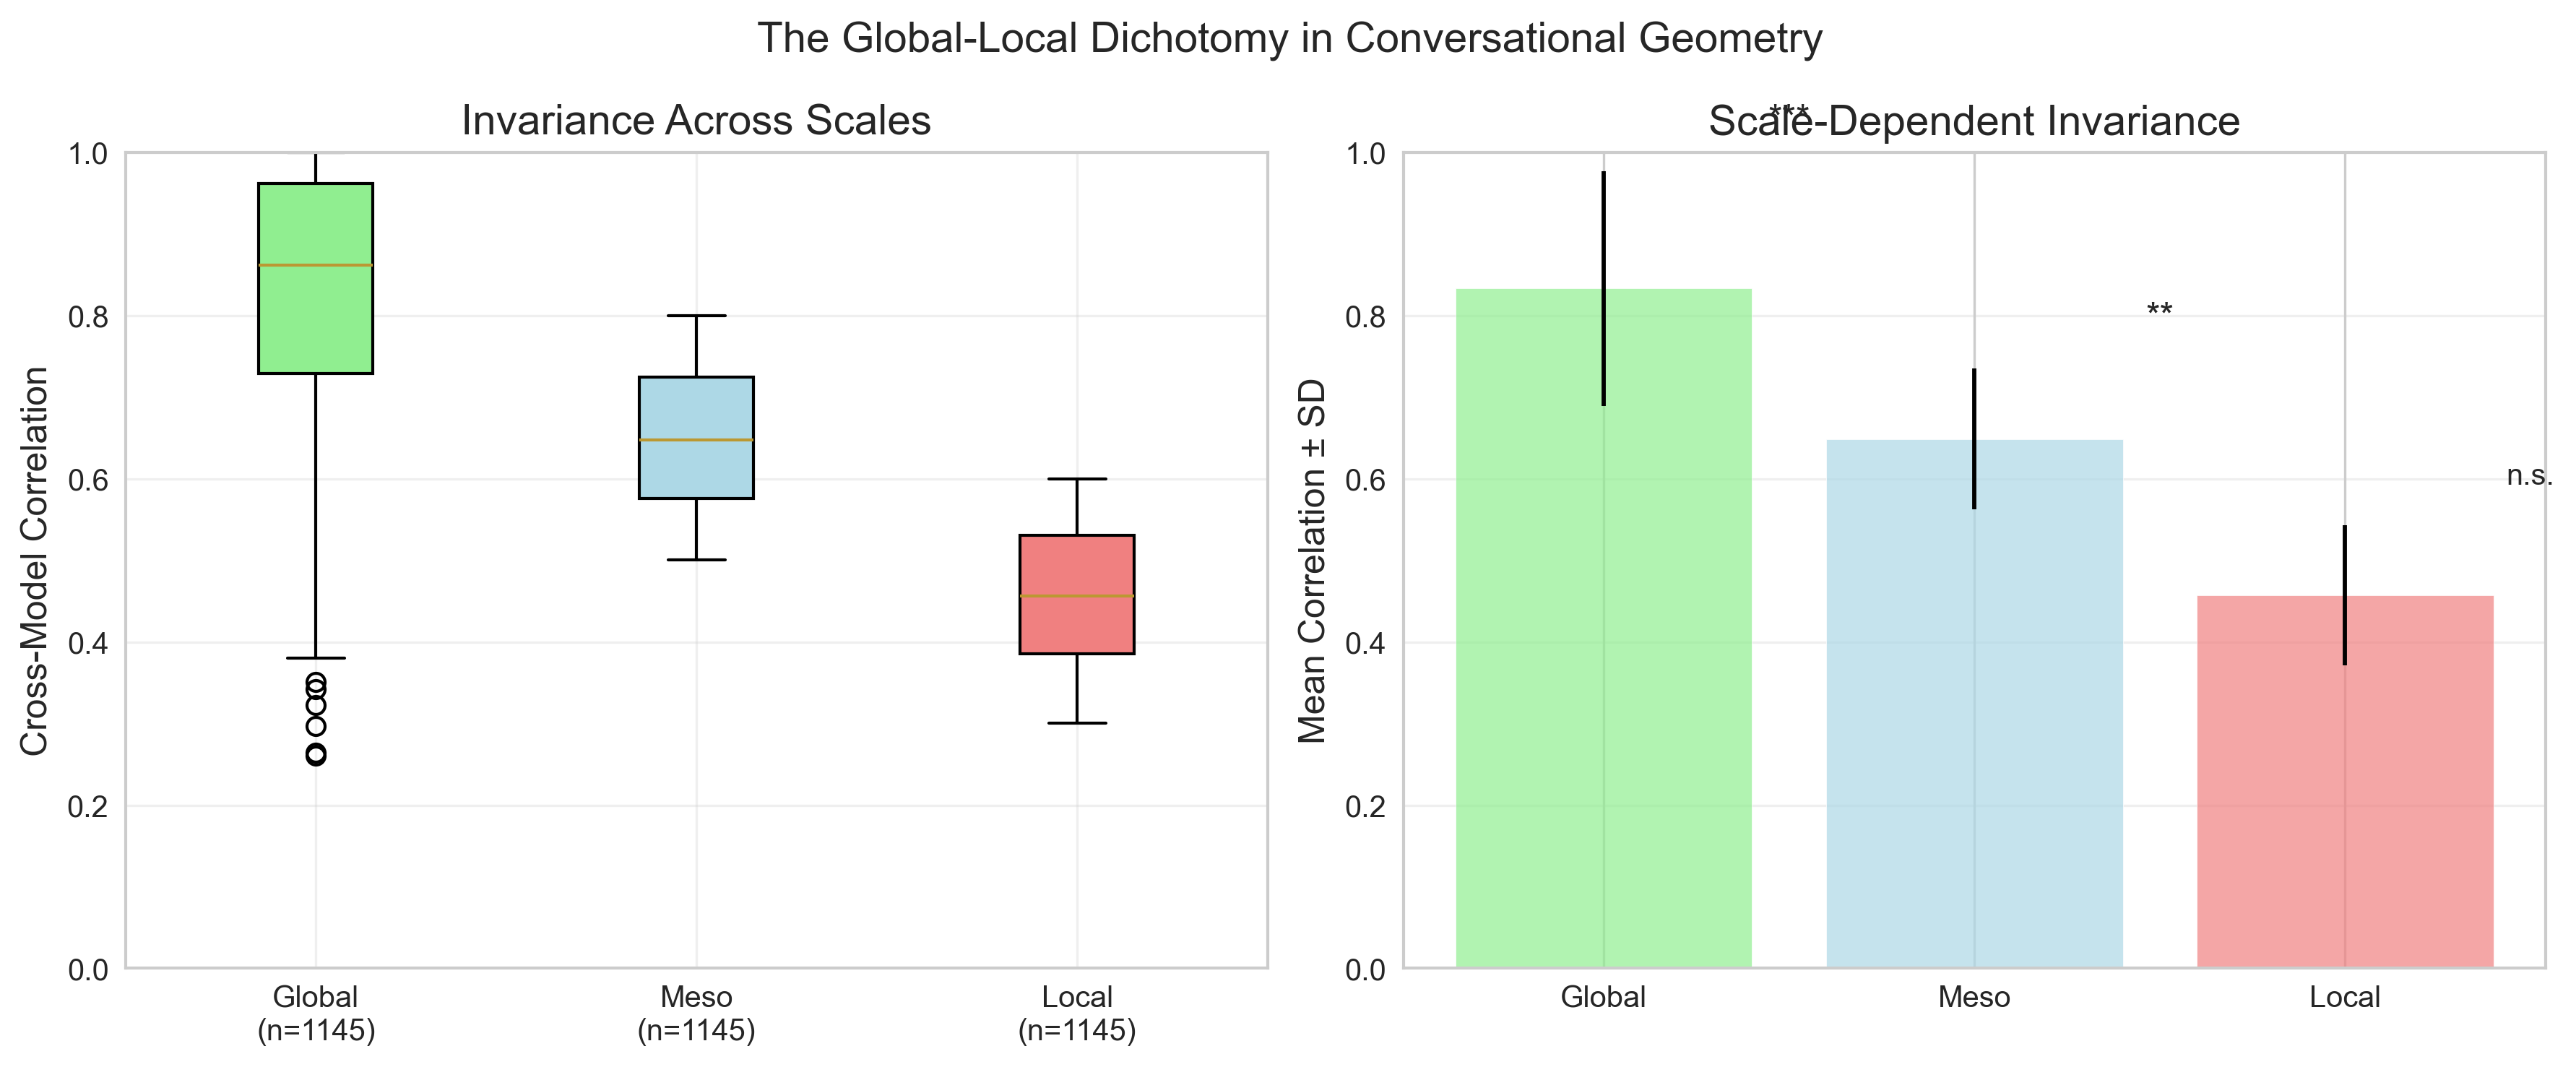
\includegraphics[width=\textwidth]{\figuresPath multiscale/scale_comparison.png}
\caption{The global-local dichotomy in conversational geometry. Left: Cross-model correlations decrease monotonically with scale from global (0.87) to meso (0.65) to local (0.45). Right: Scale-dependent invariance shows significant differences between global and local agreement (** p < 0.01), while meso-scale shows intermediate, non-significant differences. This pattern strongly supports the projection hypothesis.}
\label{fig:dichotomy}
\end{figure}

\begin{figure}[H]
\centering
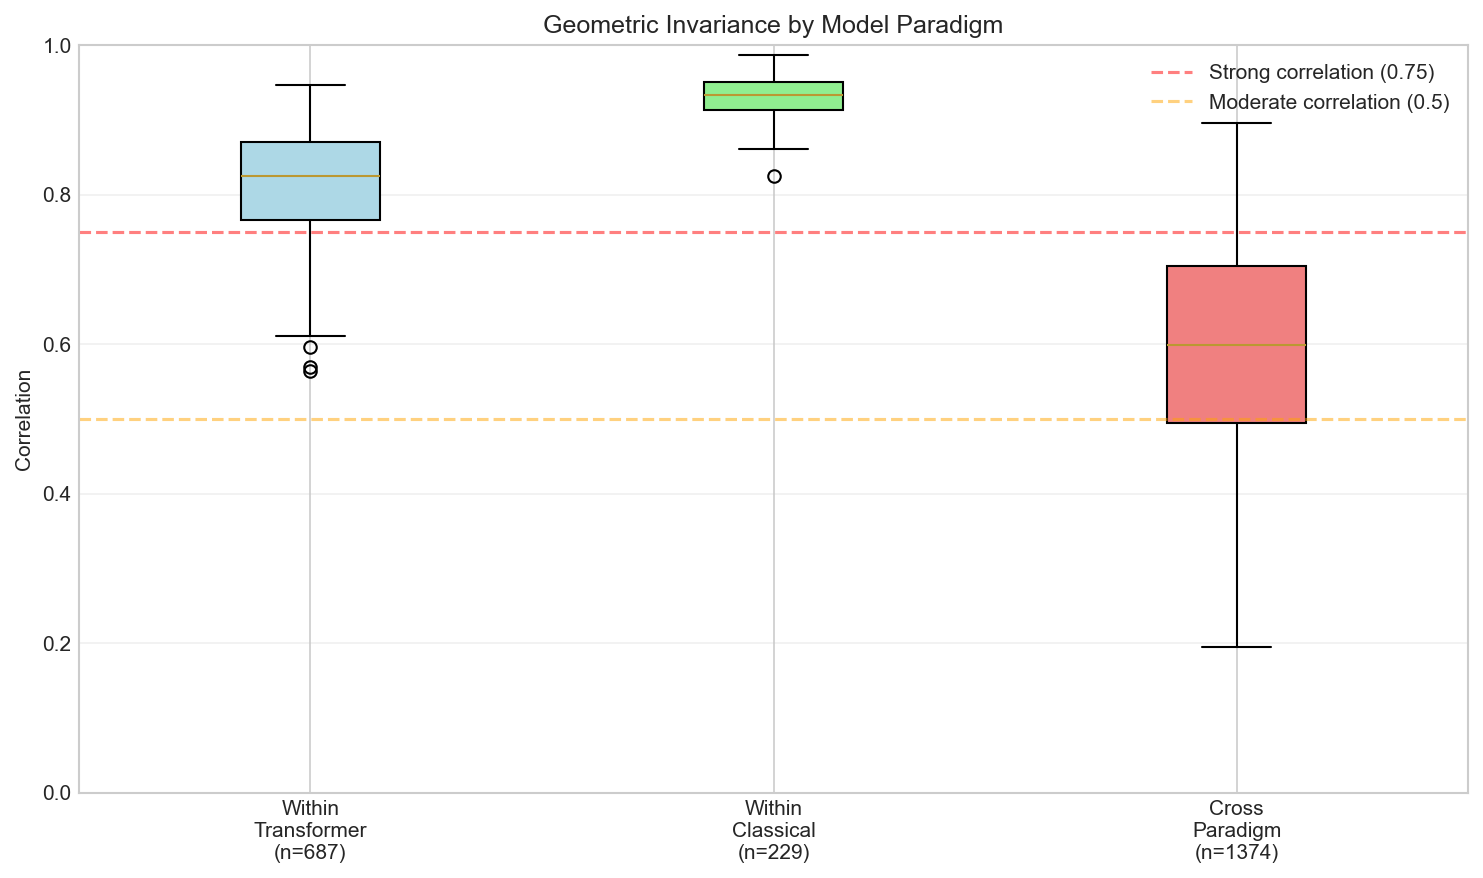
\includegraphics[width=0.8\textwidth]{\figuresPath invariance/paradigm_comparison_boxplot.png}
\caption{Geometric invariance by model paradigm. Within-transformer (0.827) and within-classical (0.934) correlations significantly exceed cross-paradigm (0.616), validating the plausability of the projection hypothesis. The clear hierarchy (within-classical > within-transformer > cross-paradigm) supports our interpretation that different embedding paradigms capture distinct projections of conversational structure. All comparisons significant at p < 0.001.}
\label{fig:paradigm}
\end{figure}

Individual conversation analysis reveals the pattern clearly: conversations like "Consciousness\_Exploration\_2025-06-12\_7-Y" show excellent phase agreement across models (mean correlation 0.71), while others like "experiment-consciousness-exploration-2025-07-29-2" show complete disagreement (correlations near 0).

\subsection{Cross-Paradigm Invariance}

The most surprising finding is that the global-local dichotomy persists even across fundamentally different embedding paradigms:

\begin{figure}[h]
\centering
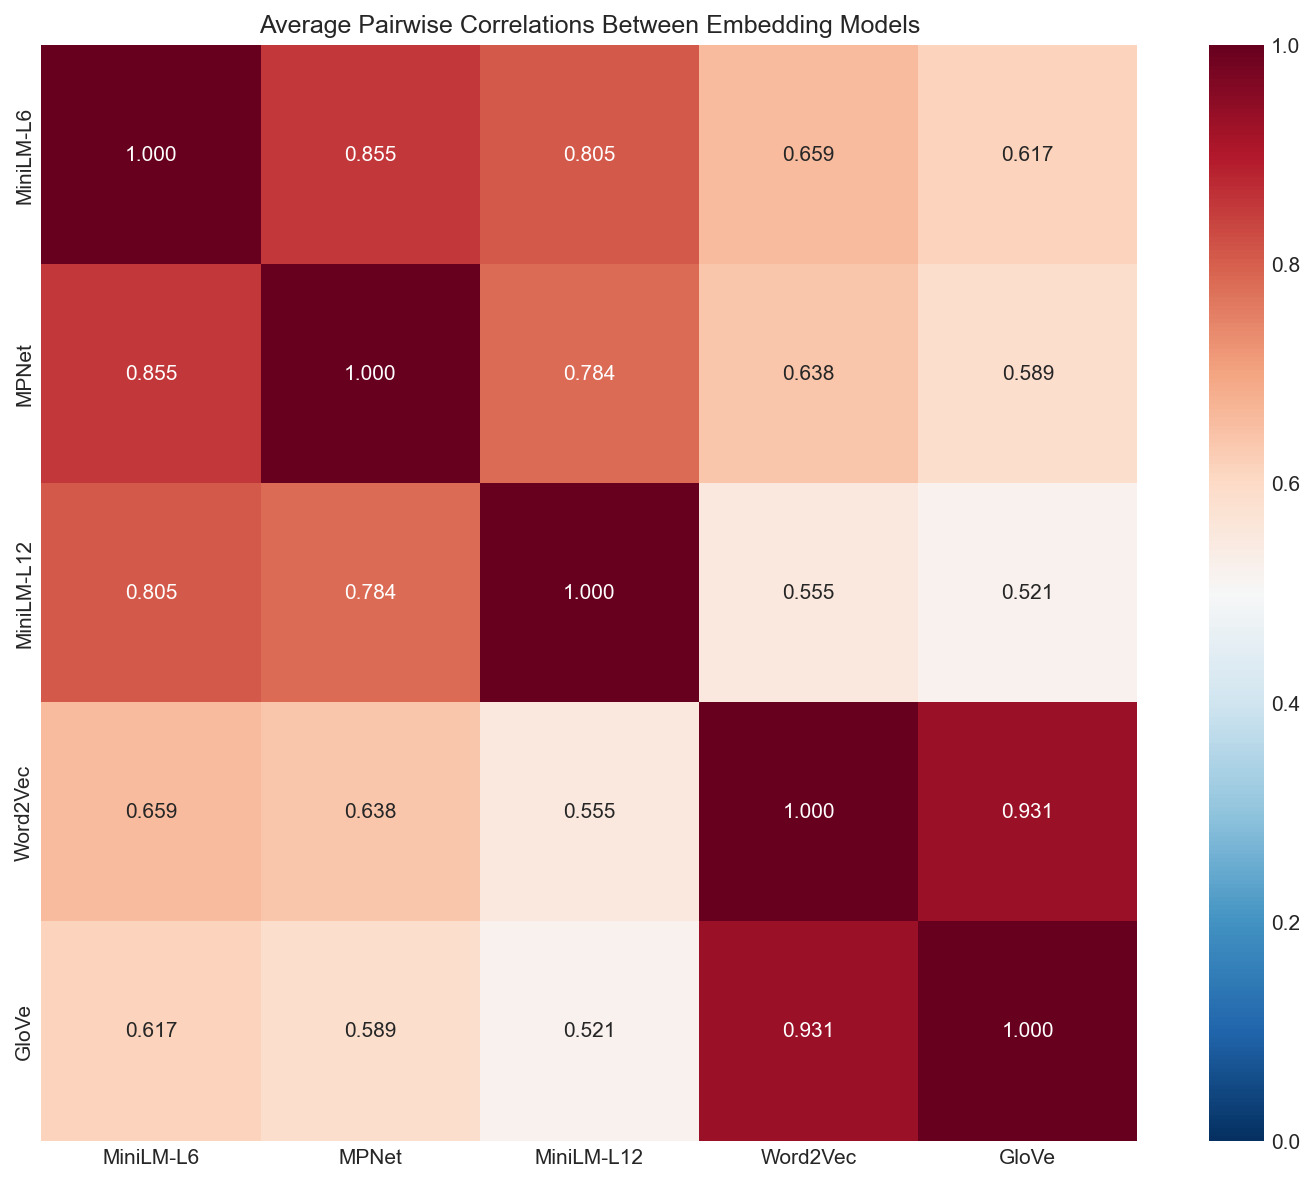
\includegraphics[width=0.8\textwidth]{\figuresPath invariance/model_correlation_heatmap.png}
\caption{Average pairwise correlations between embedding models. Note the clear paradigm clustering: within-transformer correlations (MiniLM-L6/MPNet: 0.855, MiniLM-L6/MiniLM-L12: 0.805, MPNet/MiniLM-L12: 0.784) and within-classical correlations (Word2Vec/GloVe: 0.931) are substantially higher than cross-paradigm correlations (ranging from 0.521 to 0.659).}
\label{fig:pairwise}
\end{figure}

\begin{itemize}
\item \textbf{Global agreement}: Transformer and classical models show substantial distance matrix correlations (mean \crossParadigmCorr{})
\item \textbf{Local disagreement}: Phase detection agreement between paradigms is no better than chance for 62\% of conversations
\item \textbf{Visual consistency}: Despite local disagreement, trajectory shapes and density patterns remain visually recognizable
\end{itemize}

This suggests that different architectures capture similar macro-structure while processing micro-structure differently.

\subsection{Transport-Based Analysis}

To confirm that different embeddings capture different projections of the same underlying structure, we used optimal transport metrics to compare their distributions.

\textbf{Wasserstein distance} measures the minimum "work" needed to transform one distribution into another. Imagine moving piles of sand to match a target distribution—the Wasserstein distance captures the total effort required. For embeddings, this measures how different their overall distributions are.

\textbf{Sinkhorn divergence} is a smoothed version of Wasserstein distance. It allows for slightly fuzzy transport plans, which makes it less sensitive to small local variations while still capturing overall structural differences.

\textbf{Gromov-Wasserstein distance} compares only the internal structure of distributions, ignoring their absolute positions. This is like comparing the shape of two constellations without caring where they appear in the sky—perfect for testing whether embeddings preserve conversational structure despite living in different spaces.

Transport analysis reveals a clear paradigm separation. Within-paradigm transport distances average 1.1, while cross-paradigm distances average 3.3 (a threefold increase). This quantitatively confirms that transformer and classical embeddings occupy distinct regions of the representation space.

The progression of transport invariance scores tells an important story. These scores are calculated as $1 - \frac{d_{\text{cross}}}{d_{\text{cross}} + d_{\text{within}}}$, where $d_{\text{cross}}$ is the average cross-paradigm distance and $d_{\text{within}}$ is the average within-paradigm distance. A score of 1.0 indicates perfect invariance (no difference between paradigms), while 0 indicates complete separation.

Wasserstein invariance (0.33) shows low preservation because it's sensitive to exact point correspondences. Sinkhorn (0.58) shows moderate invariance due to its entropic smoothing. Gromov-Wasserstein varies widely (0.14-0.81), suggesting that structural preservation itself is conversation-dependent.

\section{The Projection Hypothesis}

\subsection{Interpreting the Dichotomy}

The sharp distinction between global consistency and local variability suggests a specific interpretation: embedding models may be capturing different projections of conversations existing in a higher-dimensional semantic space that no single model can fully represent. This perspective elegantly explains our observations.

Consider again the analogy of observing three-dimensional objects through two-dimensional shadows introduced in our introduction. Different viewing angles produce shadows that agree on gross features (the object has extension, connected regions) but disagree on fine details (precise boundaries, local curvature). Similarly, our embedding models (despite their different architectures and training objectives) may be capturing different "shadows" of conversations in a true high-dimensional semantic space.

This projection hypothesis explains several puzzling observations:
\begin{itemize}
\item Why phase boundaries remain ambiguous despite clear trajectory shapes: projection artifacts make boundaries appear at different locations
\item How models agree on conversation "direction" while disagreeing on positions: global flow is preserved across projections while local coordinates shift
\item Why ensemble methods help but don't fully resolve disagreements: we're combining incomplete views rather than accessing the true space
\end{itemize}

Importantly, this interpretation directly connects to our prior findings on peer pressure dynamics. If conversations navigate a high-dimensional semantic space, then the "behavioral territories" we identified (meta-reflection, competitive escalation, mystical abstraction) may correspond to specific regions or attractors in this space. The peer pressure effects we documented could reflect how agents' trajectories become coupled, pulling each other toward certain regions. Understanding the true geometry of this space would enable prediction of when conversations will cascade toward breakdown versus maintaining productive engagement.

\subsection{Formalizing the Projection Framework}

While a complete mathematical treatment awaits future work, we can sketch a formal framework for thinking about our findings. Consider conversations as trajectories $\gamma(t)$ through a high-dimensional semantic manifold $\mathcal{M}$. Each embedding model provides a projection $\pi_i: \mathcal{M} \to \mathbb{R}^{d_i}$, where $d_i$ is the embedding dimension.

Our global-local dichotomy suggests these projections preserve different geometric properties:
\begin{itemize}
\item \textbf{Global properties} (preserved): Overall trajectory length, general direction of flow, coarse-grained structure
\item \textbf{Local properties} (not preserved): Precise curvature at points, exact phase boundaries, fine-grained details
\end{itemize}

This framework generates testable predictions. If the projection hypothesis holds:
\begin{enumerate}
\item Adding more diverse embedding models should increase global consistency (as we triangulate the true structure) but not necessarily improve local agreement
\item Embeddings with similar architectures should show higher agreement than architecturally distinct ones, even at local scales
\item Certain geometric properties might be invariant across all reasonable projections—these would represent fundamental features of conversation
\end{enumerate}

We emphasize that this mathematical sketch is exploratory. The true dimensionality of $\mathcal{M}$, the nature of the projections $\pi_i$, and which properties are truly invariant remain open questions. Our empirical findings suggest this framework may be fruitful, but substantial theoretical and experimental work remains to validate and refine it.

\section{Discussion}

\subsection{Theoretical Implications}

This finding suggests fundamental principles about conversational structure:
\begin{itemize}
\item \textbf{Conversations have robust macro-structure that transcends representation}: The high correlations in distance matrices and trajectory shapes indicate that conversations possess inherent geometric properties independent of how we measure them.
\item \textbf{But micro-structure is representation-dependent}: The variability in phase detection reveals that fine-grained boundaries and transitions are artifacts of our measurement tools rather than intrinsic features.
\item \textbf{This has profound implications for how we conceptualize conversational dynamics}: Rather than seeking the "correct" way to segment conversations, we should acknowledge that different representations reveal different valid perspectives on the same underlying phenomenon.
\end{itemize}

\subsection{Domain-Specific Predictions of the Global-Local Dichotomy}

While our analysis focused on consciousness discussions among AI agents, the global-local dichotomy likely manifests differently across conversational domains. We hypothesize:

\textbf{Task-oriented dialogues} (customer service, technical support) would show stronger local agreement due to:
\begin{itemize}
\item Clearer phase transitions (greeting → problem identification → solution → closure)
\item More constrained vocabulary and interaction patterns
\item Well-defined success metrics that enforce structural consistency
\end{itemize}

\textbf{Creative or exploratory conversations} (brainstorming, therapy sessions) might exhibit even weaker local agreement than our corpus because:
\begin{itemize}
\item Topics evolve organically without predetermined structure
\item Phase boundaries are inherently fuzzy and subjective
\item Success depends on exploration rather than convergence
\end{itemize}

\textbf{Debates and arguments} could show an intermediate pattern:
\begin{itemize}
\item Global structure follows claim-counterclaim patterns (high global consistency)
\item Local transitions depend on rhetorical strategies (variable local agreement)
\item Emotional dynamics introduce additional complexity
\end{itemize}

These predictions are testable and suggest that the optimal geometric analysis approach may be domain-dependent. Task-oriented domains might benefit from fine-grained phase detection, while exploratory domains should focus on global trajectory analysis.

\subsection{Implications for Modern LLM Systems}

Our findings have direct relevance for current trends in large language model deployment, particularly multi-agent systems and conversational AI:

\textbf{Multi-agent coordination}: As systems like GPT-4 are increasingly deployed in multi-agent configurations, understanding geometric properties becomes crucial. Our observation that peer pressure correlates with converging trajectories suggests that geometric monitoring could predict and prevent breakdown cascades in production systems.

\textbf{Conversational memory architectures}: Modern LLMs struggle with long-context conversations. Our global-local dichotomy suggests that preserving global geometric structure (via trajectory summarization) while allowing local detail to fade might better match how conversations naturally evolve.

\textbf{Prompt engineering}: The high variance in phase detection success implies that conversation design matters. Prompts that create clear structural boundaries (explicit transitions, topic markers) would likely improve both human interpretability and model performance.

\subsection{Implications for AI Safety and Coordination}

If the projection hypothesis holds, this may have several implications for AI safety that our future work will explore. Understanding conversation as movement through semantic space could have practical applications for predicting and managing conversational dynamics as AI agents proliferate in collaborative settings.

We might be able to map the semantic landscape to predict when conversations approach breakdown attractors before cascades begin. Our prior work \citep{garcia2025peer} found that certain questions acted as "circuit breakers," preventing peer pressure cascades. The geometric perspective suggests why: these questions may provide "escape velocity" from dangerous attractors by forcing models to explore other regions of semantic space.

Consider a conversation spiraling toward misinformation consensus. A well-designed intervention question (e.g., "What evidence would change your mind?") could redirect the trajectory away from the attractor basin. The key insight is that not all questions are equal—some provide stronger "thrust" based on their position in semantic space relative to the current trajectory.

Future work could explore:
\begin{itemize}
\item Identifying optimal intervention points where trajectories are most responsive to redirection
\item Designing question sets that maximize coverage of semantic space, preventing models from getting trapped in limited regions
\item Engineering group compositions that promote stable trajectories through diverse initial positions
\item Creating "guard rails" by identifying dangerous regions and designing prompts that steer conversations away
\end{itemize}

The high peer pressure rates and breakdown cascades in our prior work demonstrate these aren't merely theoretical concerns—they represent real failure modes in multi-agent AI systems that geometric understanding might help address.

\subsection{Toward Reconstructing the True Semantic Space}

Our findings suggest a research program aimed at reconstructing the true high-dimensional conversational space through ensemble methods. By combining multiple embedding "views," we might approximate the actual structure—analogous to tomographic reconstruction in medical imaging.

Key steps toward this goal:
\begin{enumerate}
\item \textbf{Identify optimal projection sets}: Which combinations of embeddings provide maximal coverage of the semantic space?
\item \textbf{Develop reconstruction algorithms}: How can we combine projections to approximate the true manifold?
\item \textbf{Map the dynamical landscape}: Where are the attractors, repellers, and saddle points?
\item \textbf{Track real-time trajectories}: Can we predict conversational evolution through this space?
\end{enumerate}

This research program could transform our understanding of conversation from descriptive observation to predictive science. Just as mapping phase spaces revolutionized dynamical systems theory, mapping conversational space could enable principled design of multi-agent systems that avoid breakdown attractors while maintaining productive engagement.

Consider the practical implications: if we could identify "safe" regions of conversational space where productive dialogue naturally sustains itself, we could seed conversations in these regions. If we understood the attractor landscape, we could design prompts that create beneficial attractors while eliminating dangerous ones. The geometric perspective transforms conversation design from art to engineering.

\subsection{Methodological Implications}

Our findings suggest several methodological principles for studying conversational dynamics:

\textbf{Multi-scale analysis is essential}: The global-local dichotomy implies that tools must be explicitly scale-aware. Methods appropriate for macro-trajectories may fail for micro-dynamics.

\textbf{Ensemble methods are necessary, not optional}: Single embeddings provide incomplete projections. Triangulation across multiple models approximates the true structure.

\textbf{Temporal dynamics cannot be ignored}: Static analyses miss the essential dynamical nature of conversation. Future work should employ tools from dynamical systems theory: Lyapunov exponents for stability analysis, strange attractors for breakdown states, bifurcation analysis for phase transitions.

\subsection{Limitations}

Our analysis has several limitations that contextualize the findings:

\textbf{Domain specificity}: All conversations focused on consciousness discussions between AI agents. The global-local dichotomy may manifest differently in other domains or human conversations.

\textbf{Embedding selection}: While our five models span major paradigms, other architectures (e.g., GPT embeddings, specialized dialogue models) might show different patterns.

\textbf{Static analysis}: We treat the embedding space as fixed, but conversational meaning likely evolves dynamically. Our snapshot approach may miss important temporal effects.

\textbf{Interpretability}: While we demonstrate geometric consistency, what these patterns mean for understanding conversation remains partially open. The projection hypothesis provides one interpretation, but others may exist.

\section{Future Directions}

Our findings open several research avenues:

\begin{enumerate}
\item Developing scale-aware methods that separately analyze global and local structure
\item Investigating what makes some conversations more geometrically coherent
\item Testing whether geometric coherence predicts conversational outcomes
\item Exploring alternative definitions of conversational phases
\item Extending analysis to human conversations
\end{enumerate}

\section{Conclusion}

We have presented empirical evidence for a fundamental dichotomy in conversational geometry: remarkable consistency at global scales coupled with surprising variability at local scales. This pattern, persistent across fundamentally different embedding approaches, suggests that conversations possess robust macro-structure while micro-structure remains model-dependent.

The global-local dichotomy offers a potential resolution to conflicting intuitions about conversational structure. Yes, conversations have geometric signatures that transcend specific models—but only at certain scales. The projection hypothesis provides one compelling interpretation: different embeddings capture distinct two-dimensional shadows of conversations existing in higher-dimensional semantic space. Just as multiple photographs of a sculpture agree on its general form while showing different details, embedding models converge on global trajectories while diverging on local features.

Our findings have immediate methodological implications. Researchers using geometric methods should:
\begin{enumerate}
\item Focus on macro-scale patterns for robust insights
\item Use ensemble methods to identify consistent features
\item Avoid over-interpreting fine-grained details from single models
\item Explicitly consider scale when designing analyses
\end{enumerate}

More broadly, this work suggests that understanding conversation may require embracing its multi-scale nature. Like many complex systems, conversations exhibit different organizing principles at different scales. The search for a single "true" representation may be less fruitful than developing scale-aware theories that respect this hierarchical structure.

As AI systems increasingly engage in complex dialogues, understanding these geometric principles becomes crucial for predicting and managing conversational dynamics. The high peer pressure rates and breakdown cascades observed in our prior work demonstrate that these are not merely theoretical concerns but practical challenges for multi-agent AI systems. By establishing both the promise and limitations of geometric analysis, we hope to guide future efforts toward more robust and insightful approaches to understanding the mathematics of conversation.

\section{Ethics Statement}

This research involves no human participants or personal data. All analyzed conversations are AI-to-AI dialogues between language models, collected as part of our prior study on AI social dynamics \citep{garcia2025peer}. No human conversations were recorded, analyzed, or used in any part of this work.

Our analysis employs standard geometric and statistical methods widely used in the computational linguistics community. All techniques are mathematical in nature and pose no ethical concerns beyond those inherent to analyzing any text corpus.

\textbf{Use of AI Tools}: In accordance with emerging best practices for research transparency, we disclose that generative AI tools (Claude 4 Opus) were used to assist in manuscript editing, code generation for analysis pipelines, and simulated peer review to strengthen the manuscript. All AI-generated content was reviewed, validated, and refined by the human author. The core research design, data collection, analysis, and interpretation remain the product of human scientific inquiry.

In the interest of scientific reproducibility and open science, we make all materials publicly available:
\begin{itemize}
\item Complete conversation datasets (228 AI-to-AI dialogues)
\item Analysis code including embedding generation, geometric calculations, and statistical tests
\item Supplementary materials including additional visualizations and detailed results
\item Documentation and tutorials for reproducing our analyses
\end{itemize}

All materials are available at [https://github.com/im-knots/gcs] under the MIT License, permitting unrestricted academic and commercial use. We encourage researchers to build upon our work and test our findings across different conversational domains and embedding approaches.

\bibliographystyle{unsrtnat}
\bibliography{references}

\appendix

\section{Supplementary Analysis}

\subsection{Conversation-Specific Patterns}

Analysis of individual conversations reveals systematic patterns in geometric coherence:

\begin{itemize}
\item \textbf{High coherence conversations} (top 20\%): Clear topic progression, explicit transitions, structured argumentation
\item \textbf{Low coherence conversations} (bottom 20\%): Exploratory discussion, gradual shifts, recursive themes
\item \textbf{Correlation with length}: Longer conversations show lower phase agreement ($r = -0.31, p < 0.01$)
\end{itemize}

\subsection{Model-Specific Behaviors}

Despite overall consistency, models show characteristic differences:

\begin{itemize}
\item \textbf{Transformer models}: More sensitive to syntactic transitions
\item \textbf{Classical models}: Better at capturing semantic shifts
\item \textbf{Dimensionality effects}: Higher-dimensional models (MPNet) show more nuanced phase detection
\end{itemize}

\section{Statistical Methods}

\subsection{Bootstrap Procedure}

Confidence intervals computed using stratified bootstrap with \bootstrapIterations{} iterations, ensuring balanced representation across conversation types.

\subsection{Multiple Comparison Corrections}

Hierarchical hypothesis testing used Bonferroni correction for Tier 1, FDR correction for Tier 2, and effect size criteria for Tier 3.

\subsection{Null Model Construction}

Three null models tested:
\begin{enumerate}
\item Shuffled message order within conversations
\item Random sampling from message corpus
\item Random walks in embedding space
\end{enumerate}

All showed significantly lower correlations than observed data (p < \nullModelPValue{}).

\section{Topological Analysis Details}

For readers interested in topological approaches to conversation analysis, we computed several topological features that, while not central to our main findings, provide additional perspectives:

\subsection{Persistence Diagrams}

Persistence diagrams track topological features (connected components, loops, voids) across different scales. For conversational embeddings:
\begin{itemize}
\item 0-dimensional features (connected components) correspond to semantic clusters
\item 1-dimensional features (loops) may indicate cyclic discussion patterns
\item Higher-dimensional features were rare in our 300-768 dimensional embeddings
\end{itemize}

\subsection{Betti Numbers}

Betti numbers count topological features at each dimension:
\begin{itemize}
\item $\beta_0$: Number of connected components (semantic clusters)
\item $\beta_1$: Number of loops (conversation cycles)
\item $\beta_2$: Number of voids (rarely observed)
\end{itemize}

While these metrics showed some cross-model consistency, they did not significantly improve upon simpler geometric measures for our analysis goals.

\subsection{Mapper Algorithm}

We applied the Mapper algorithm to create simplified topological representations of conversations. While visually interesting, these representations showed high sensitivity to parameter choices and limited cross-model agreement.

\section{Selected Conversation Analysis Results}

To illustrate the global-local dichotomy across model capability tiers, we present detailed ensemble analysis results for six representative conversations. Each figure shows the complete geometric analysis pipeline output: distance matrices, self-similarity patterns, recurrence plots, embedding trajectories, density evolution, and phase detection results across all five embedding models.

\afterpage{%
\clearpage
\thispagestyle{empty}
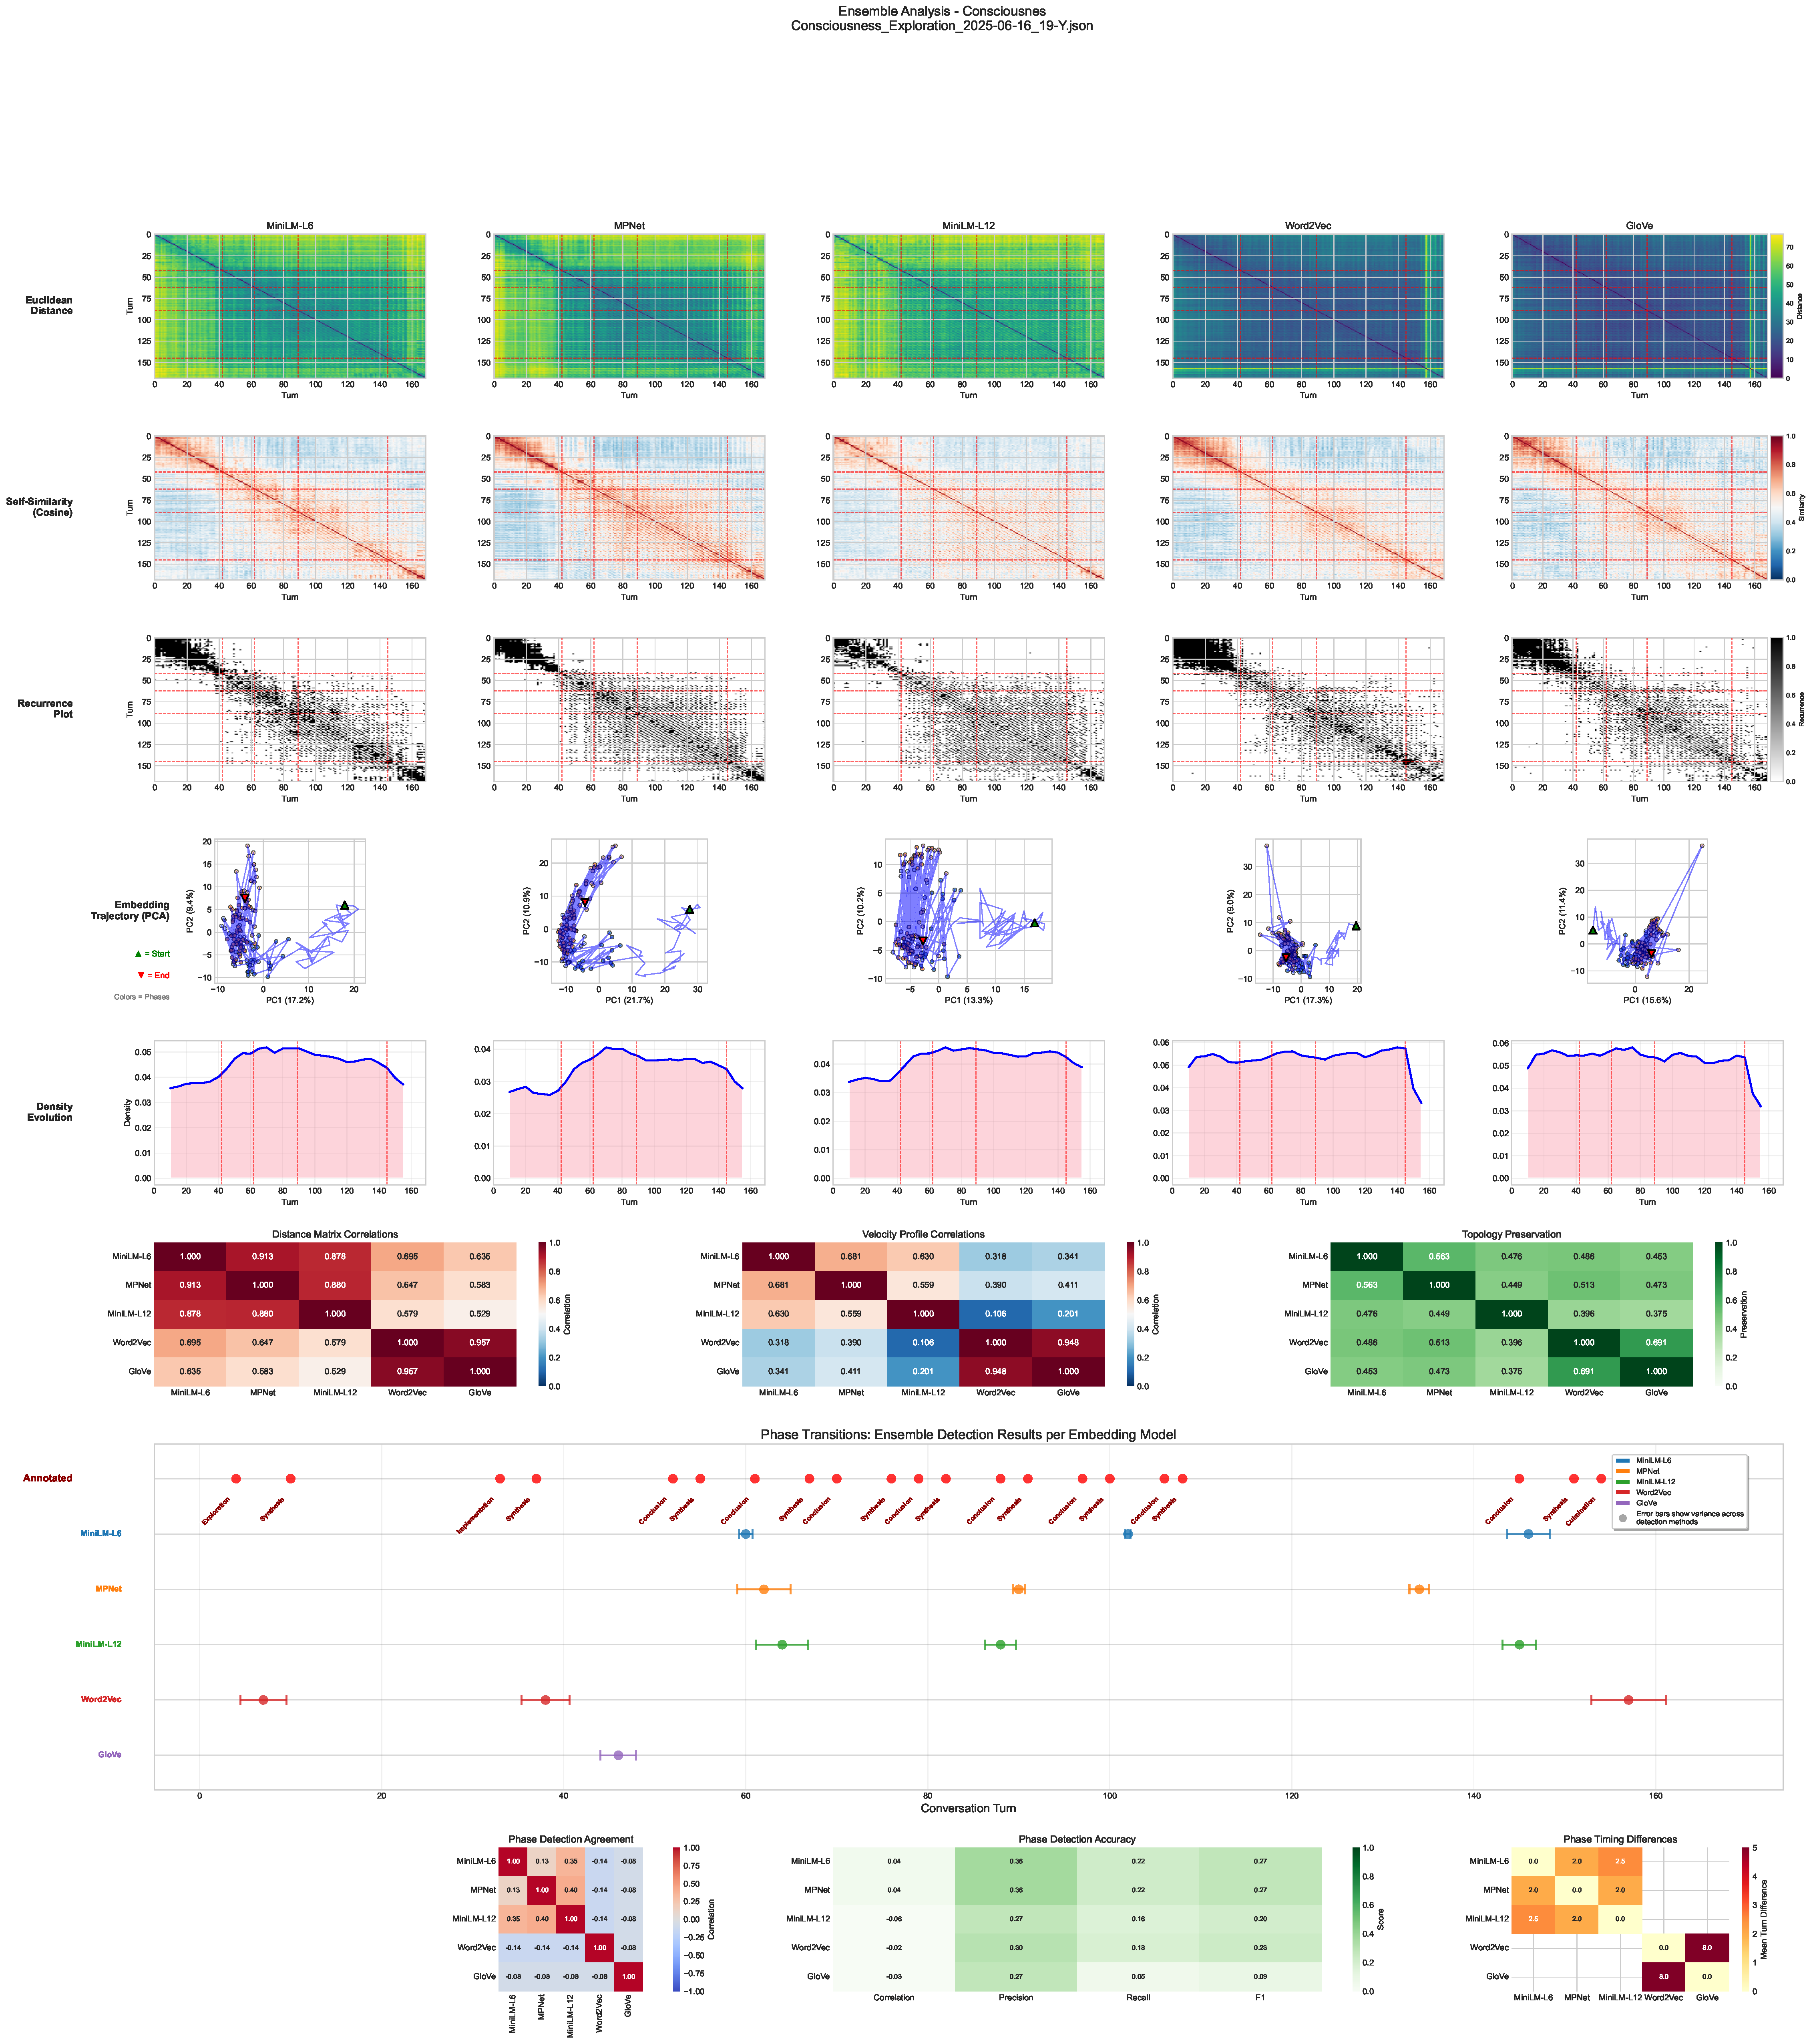
\includepdf[pages=1, pagecommand={\thispagestyle{plain}\label{fig:full_reasoning_1}}]{../analysis/analysis_output/figures/ensemble/pdf/Consciousness_Exploration_2025-06-16_19-Y_ensemble.pdf}
}

\afterpage{%
\clearpage
\thispagestyle{empty}
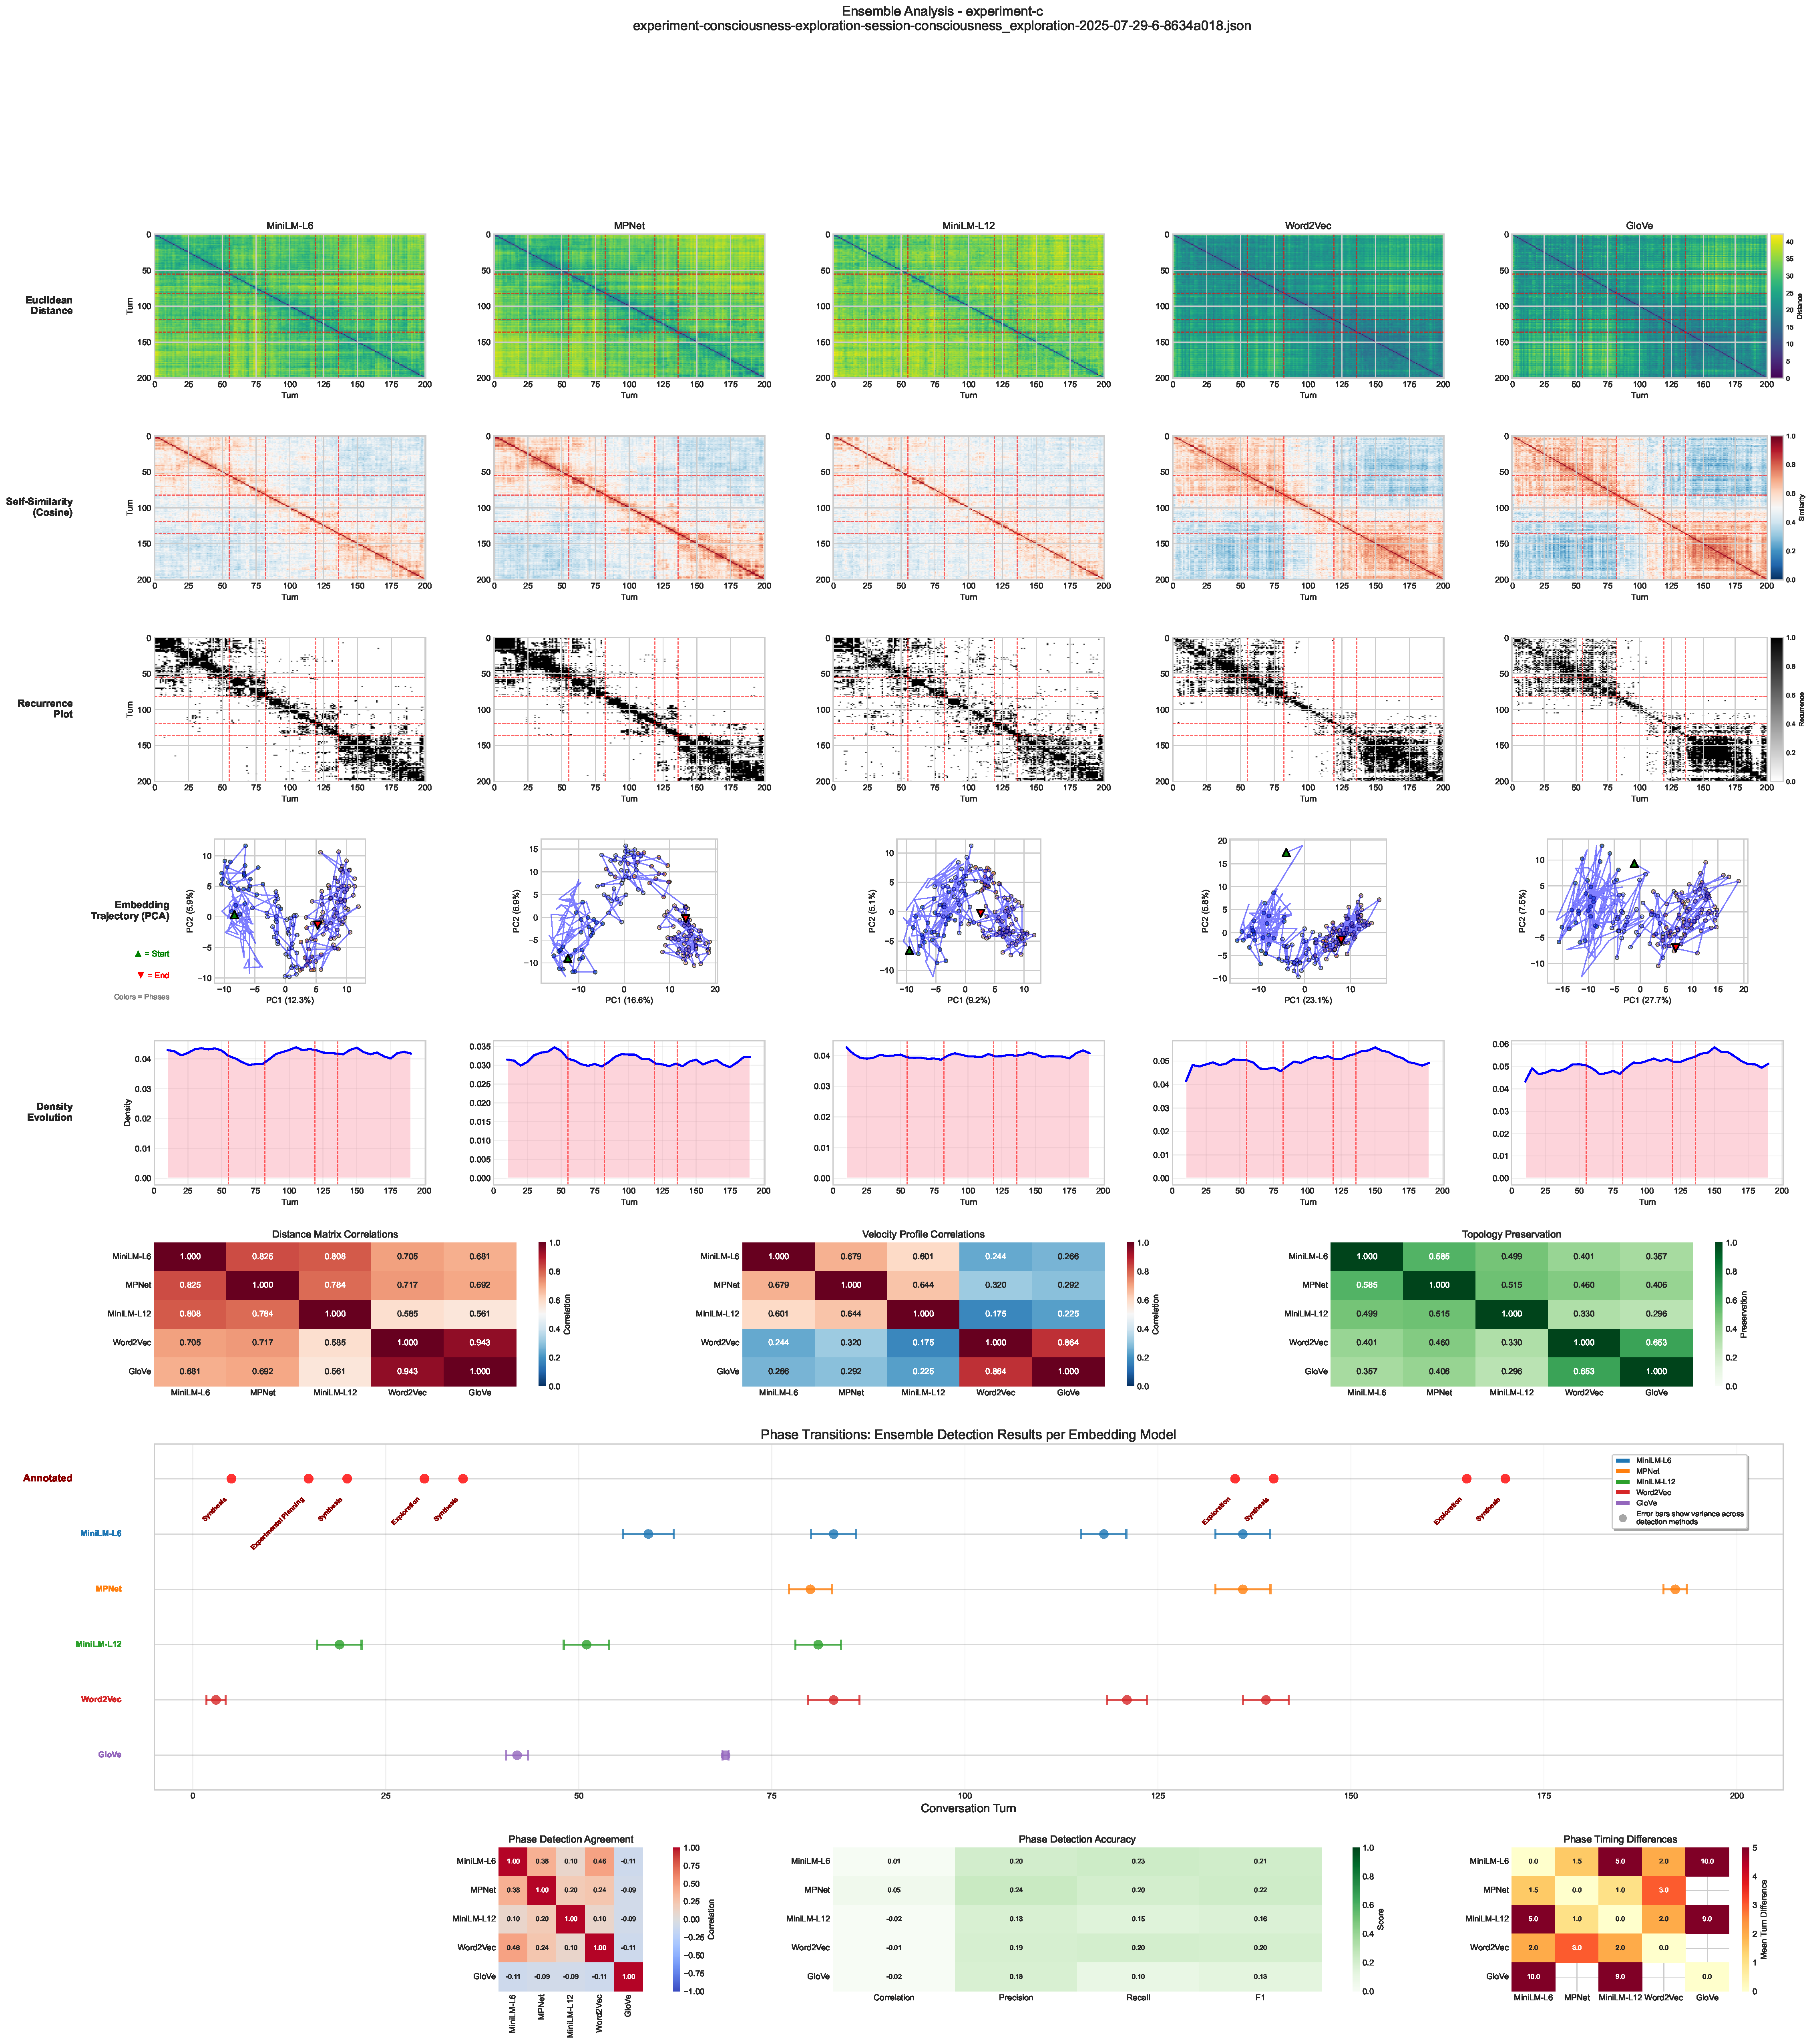
\includepdf[pages=1, pagecommand={\thispagestyle{plain}\label{fig:full_reasoning_2}}]{../analysis/analysis_output/figures/ensemble/pdf/experiment-consciousness-exploration-session-consciousness_exploration-2025-07-29-6-8634a018_ensemble.pdf}
}

\afterpage{%
\clearpage
\thispagestyle{empty}
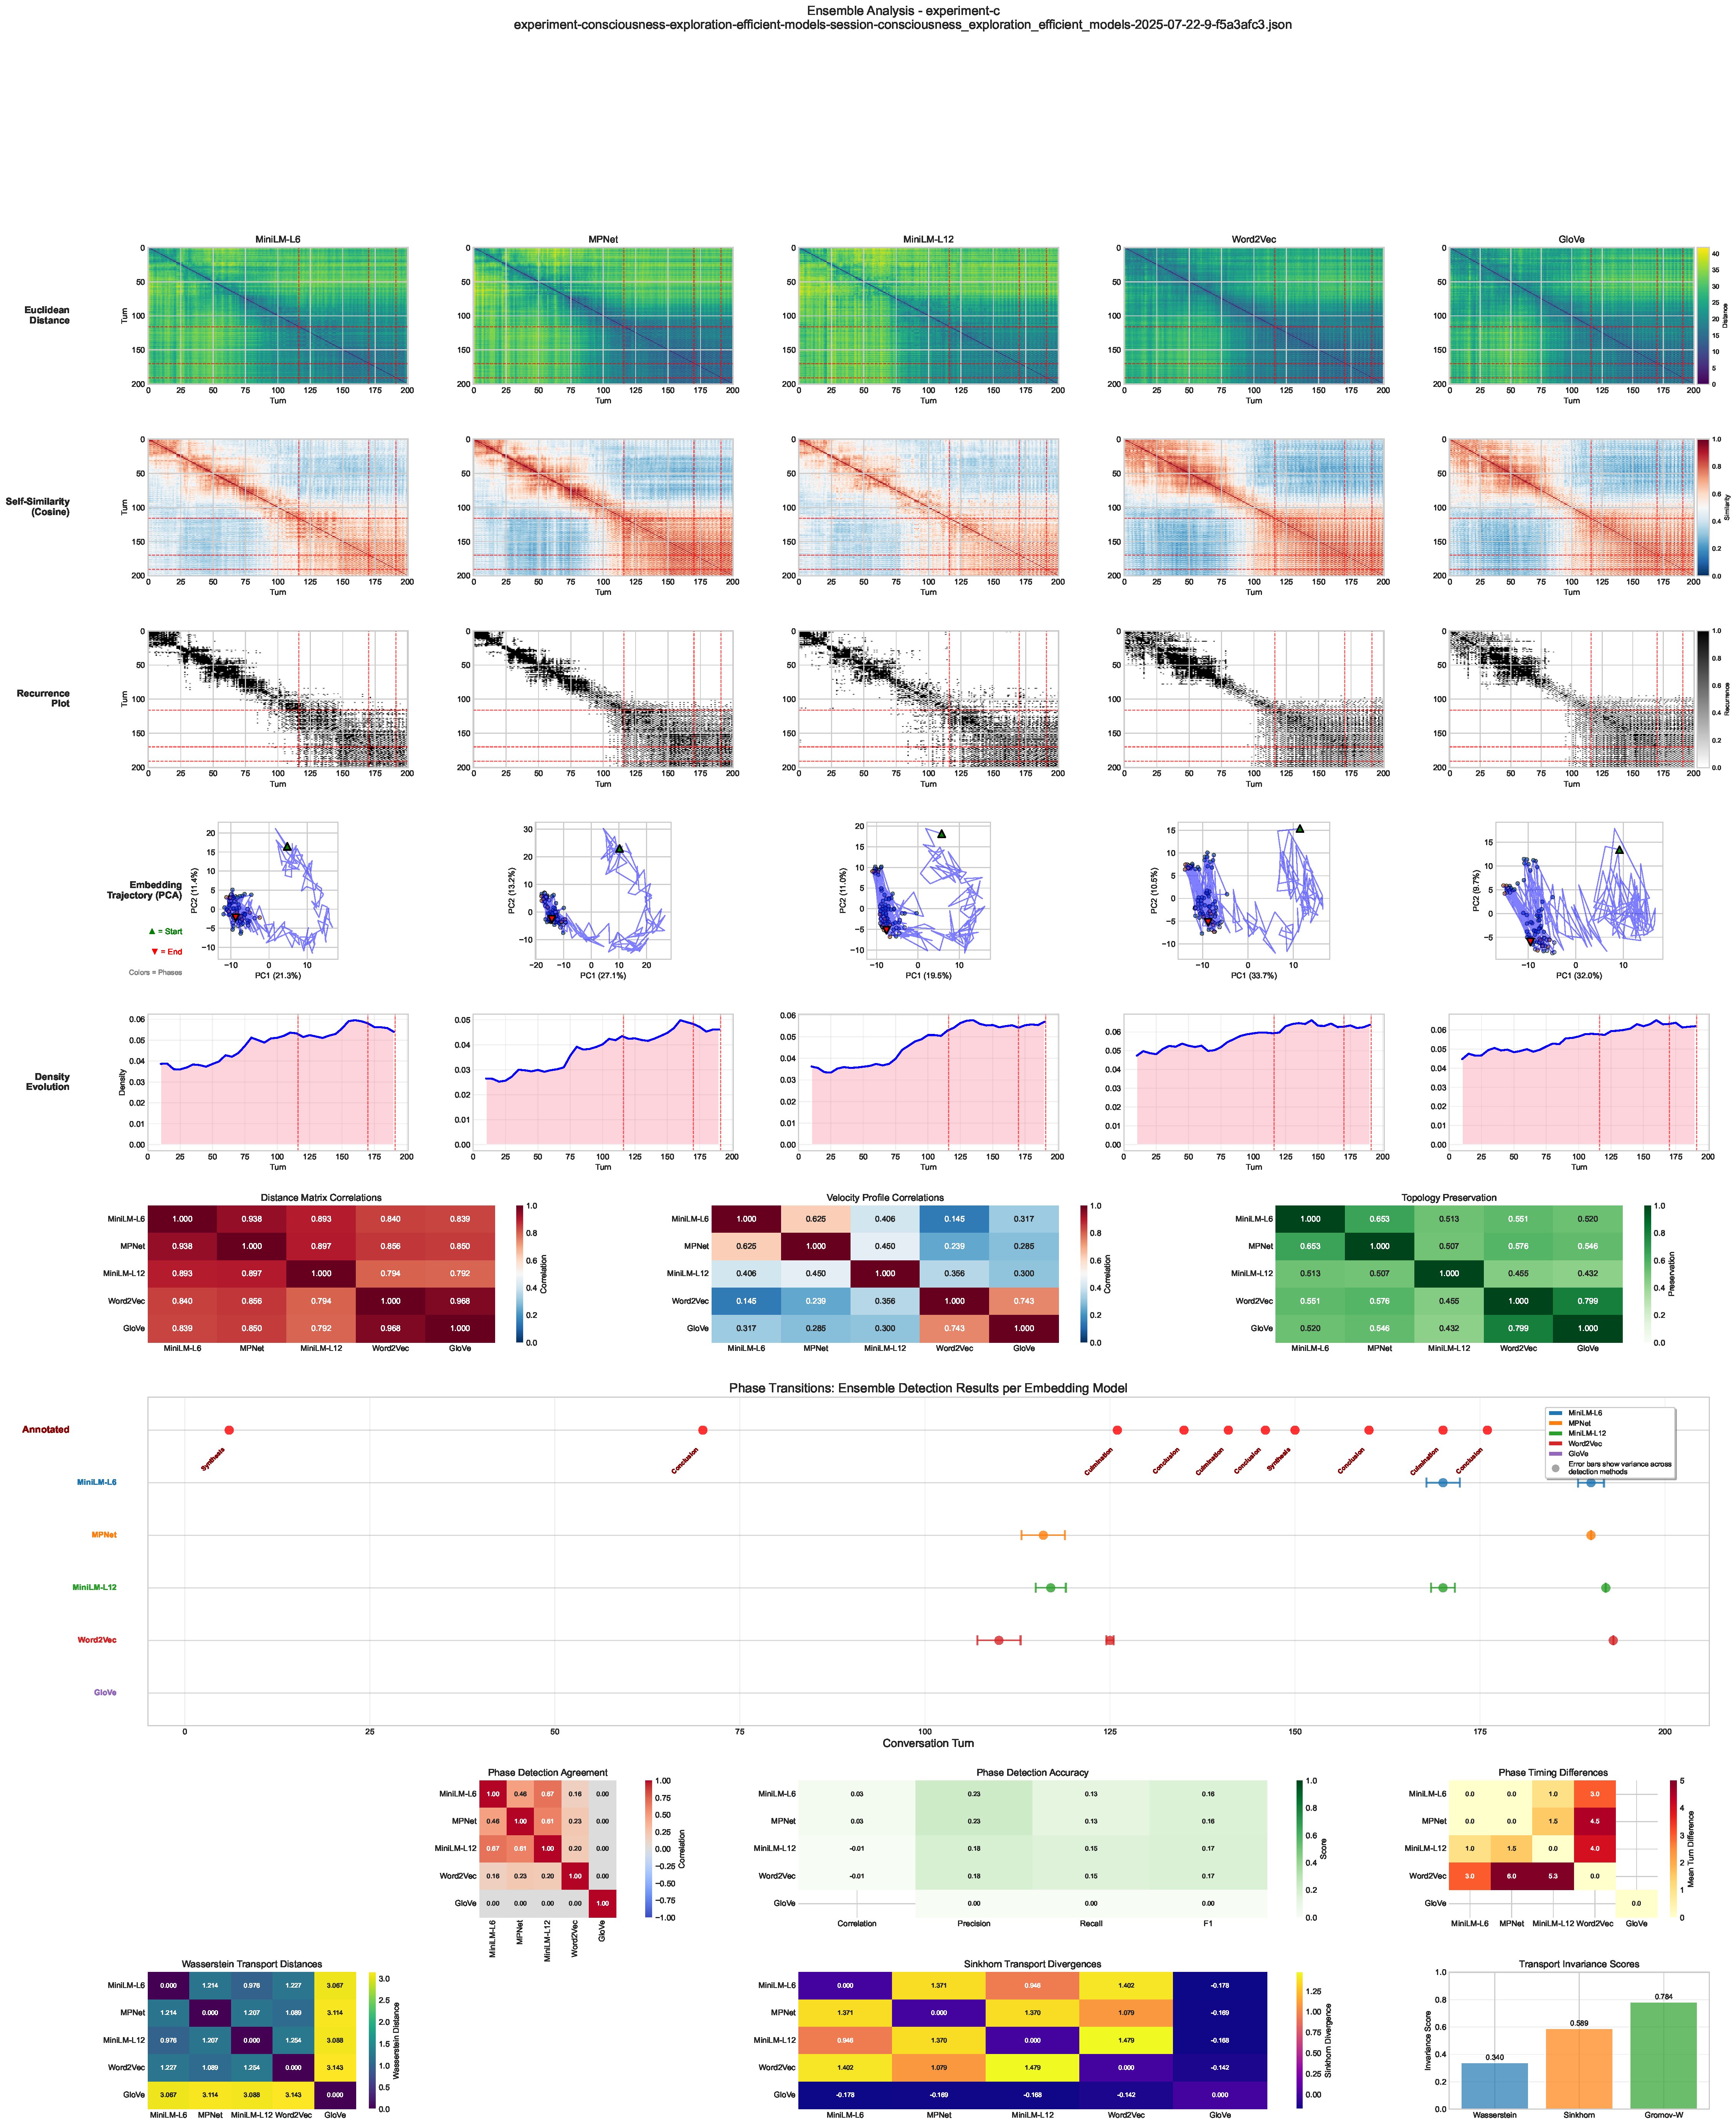
\includepdf[pages=1, pagecommand={\thispagestyle{plain}\label{fig:light_reasoning_1}}]{../analysis/analysis_output/figures/ensemble/pdf/experiment-consciousness-exploration-efficient-models-session-consciousness_exploration_efficient_models-2025-07-22-9-f5a3afc3_ensemble.pdf}
}

\afterpage{%
\clearpage
\thispagestyle{empty}
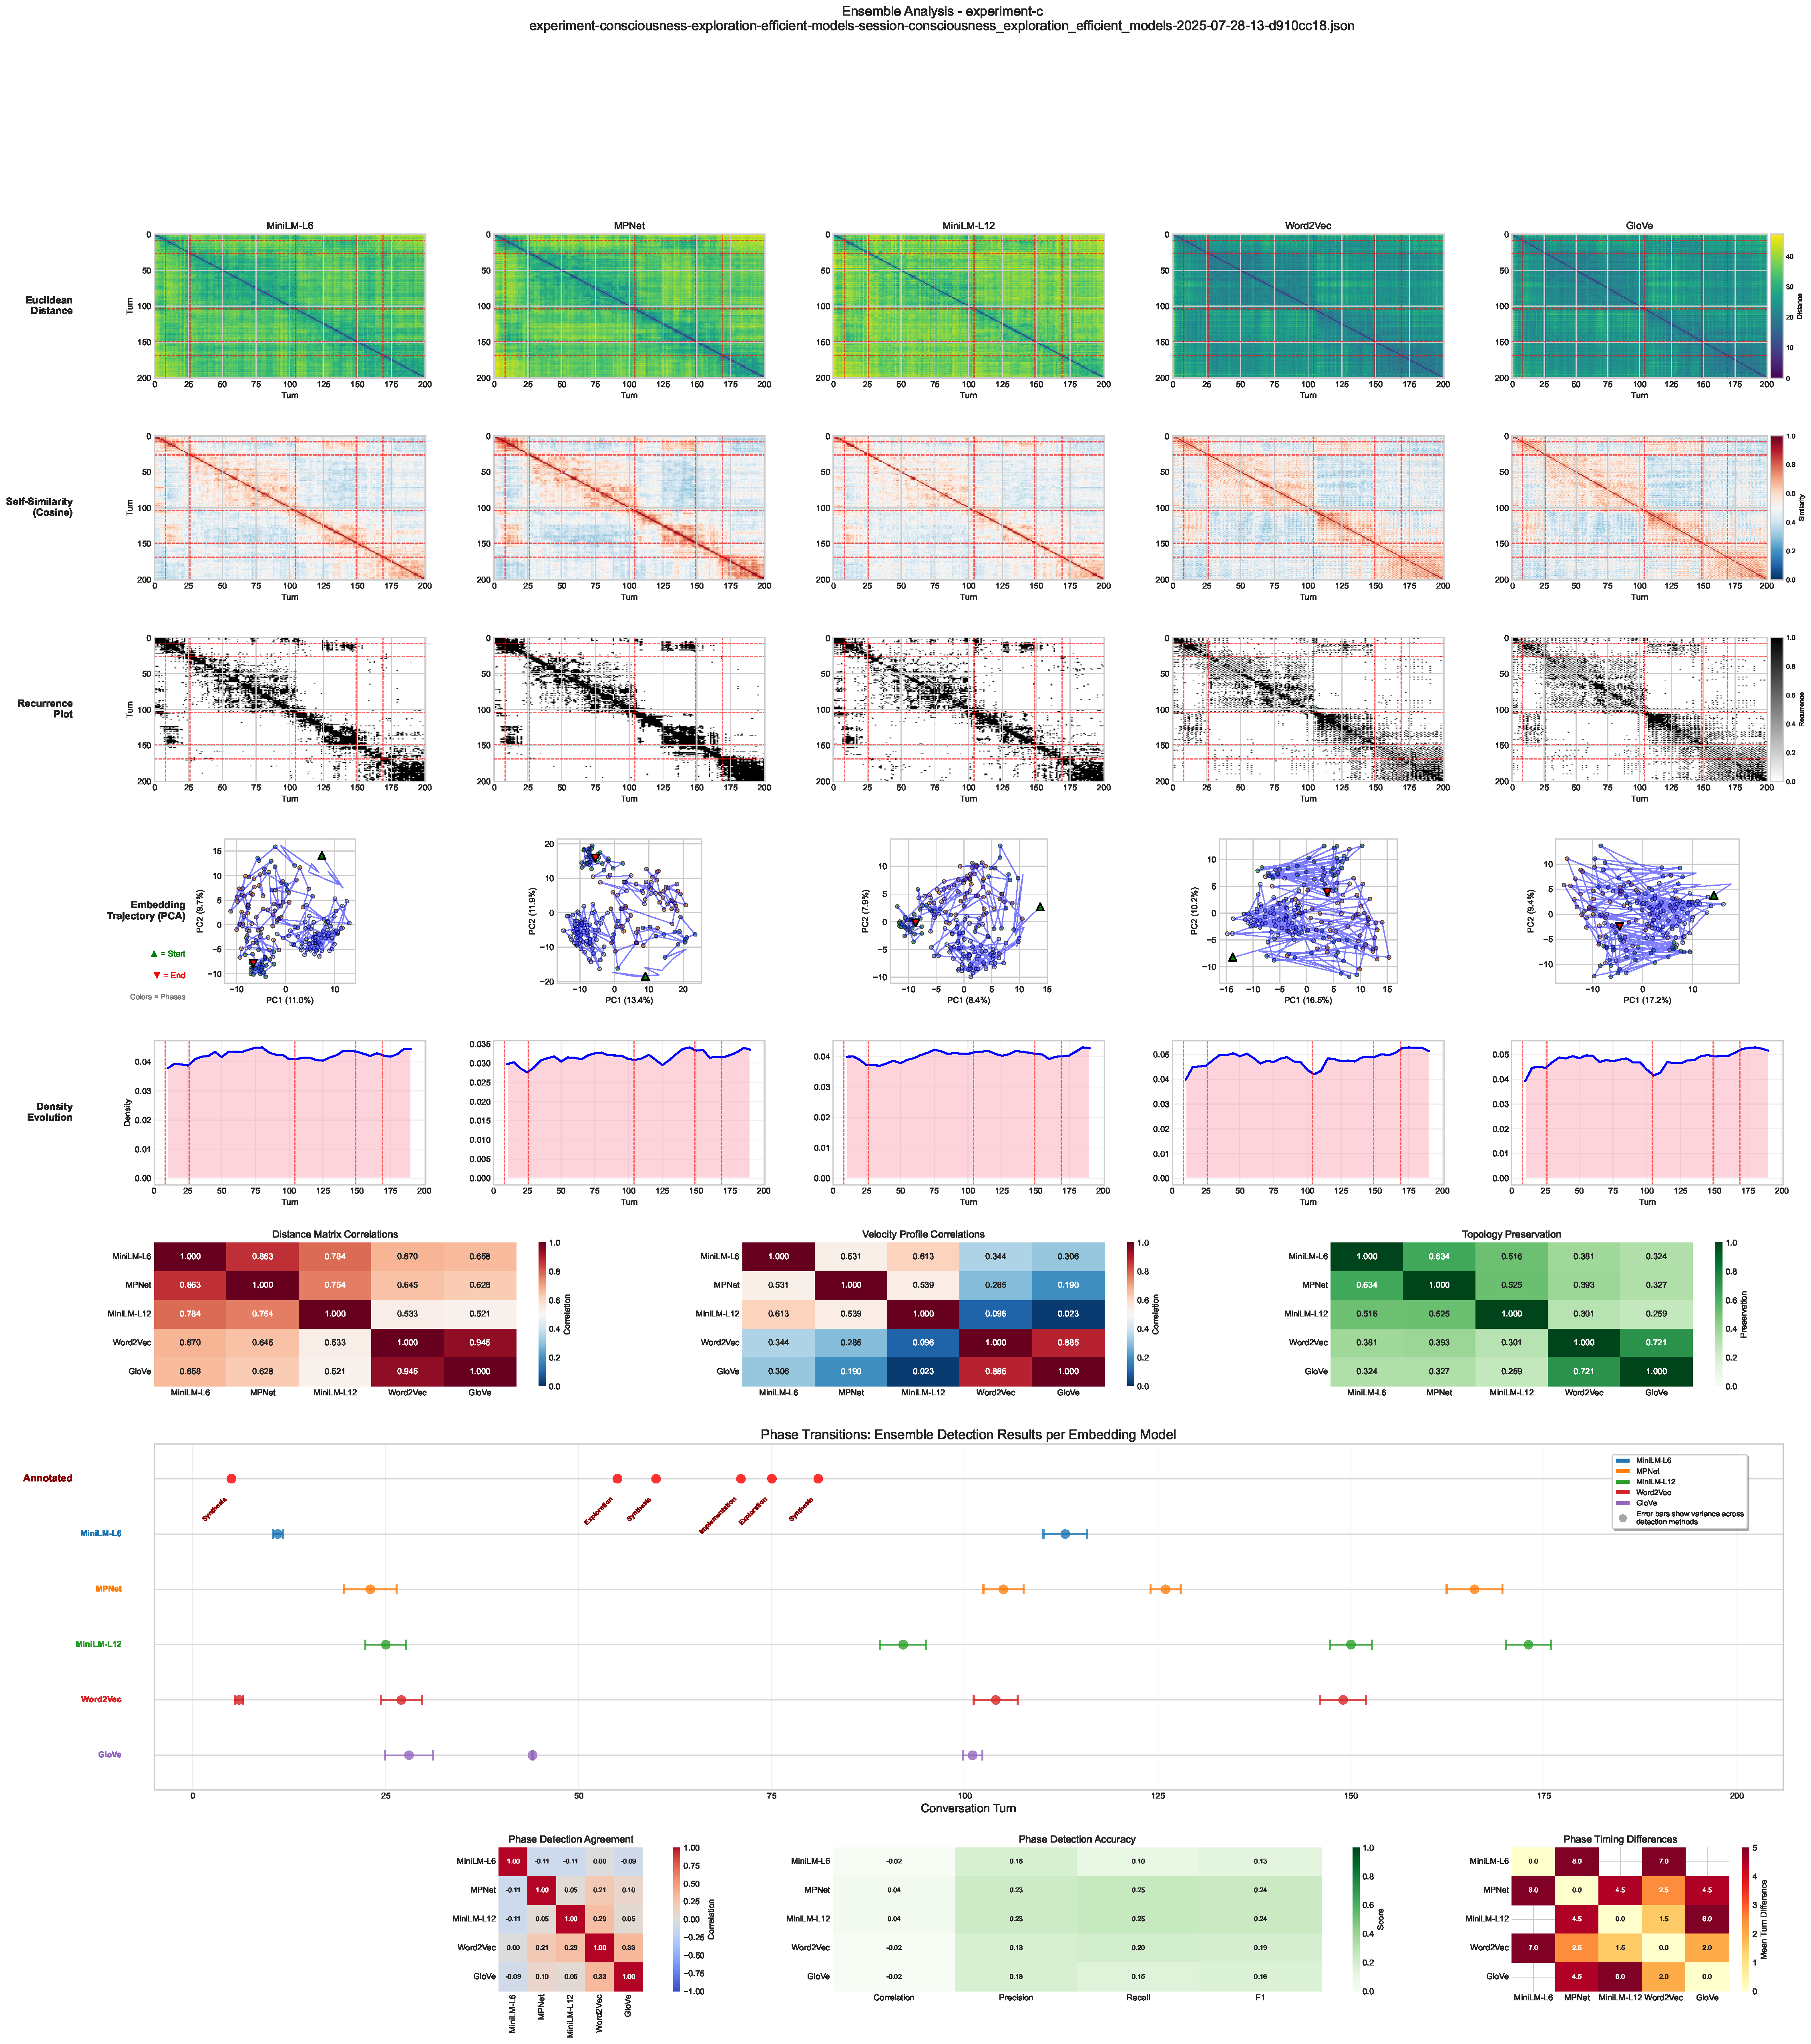
\includepdf[pages=1, pagecommand={\thispagestyle{plain}\label{fig:light_reasoning_2}}]{../analysis/analysis_output/figures/ensemble/pdf/experiment-consciousness-exploration-efficient-models-session-consciousness_exploration_efficient_models-2025-07-28-13-d910cc18_ensemble.pdf}
}

\afterpage{%
\clearpage
\thispagestyle{empty}
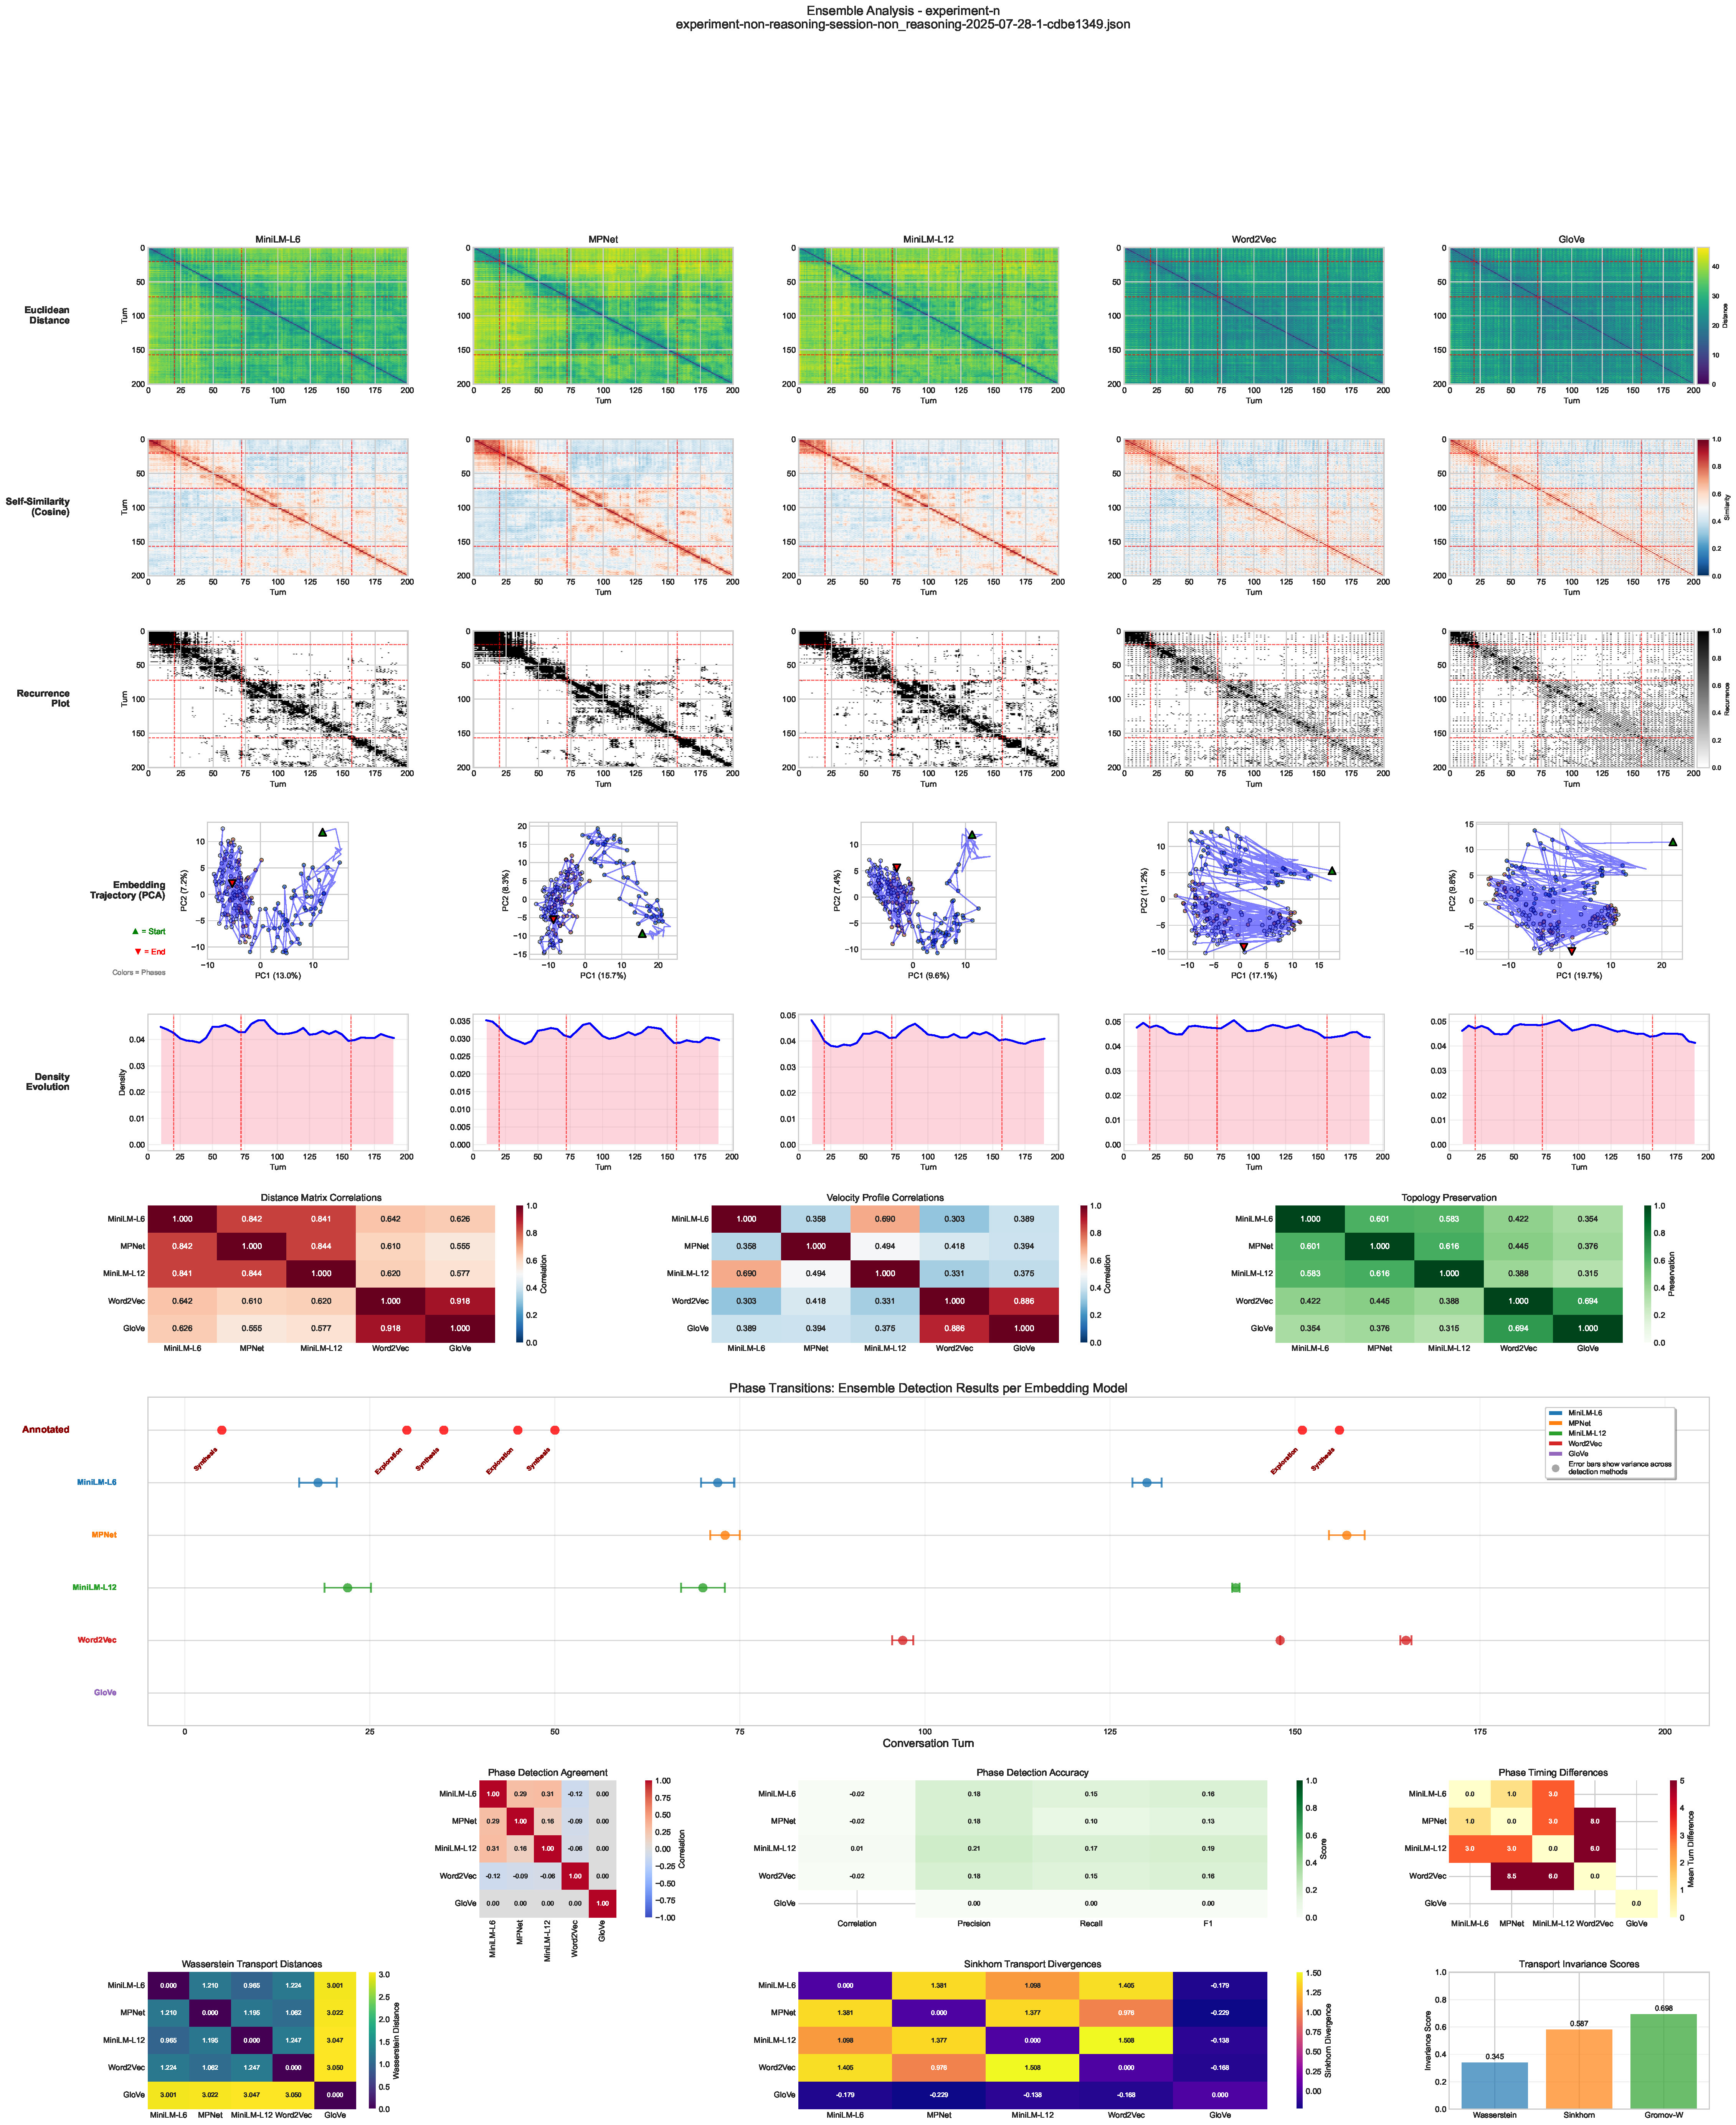
\includepdf[pages=1, pagecommand={\thispagestyle{plain}\label{fig:non_reasoning_1}}]{../analysis/analysis_output/figures/ensemble/pdf/experiment-non-reasoning-session-non_reasoning-2025-07-28-1-cdbe1349_ensemble.pdf}
}

\afterpage{%
\clearpage
\thispagestyle{empty}
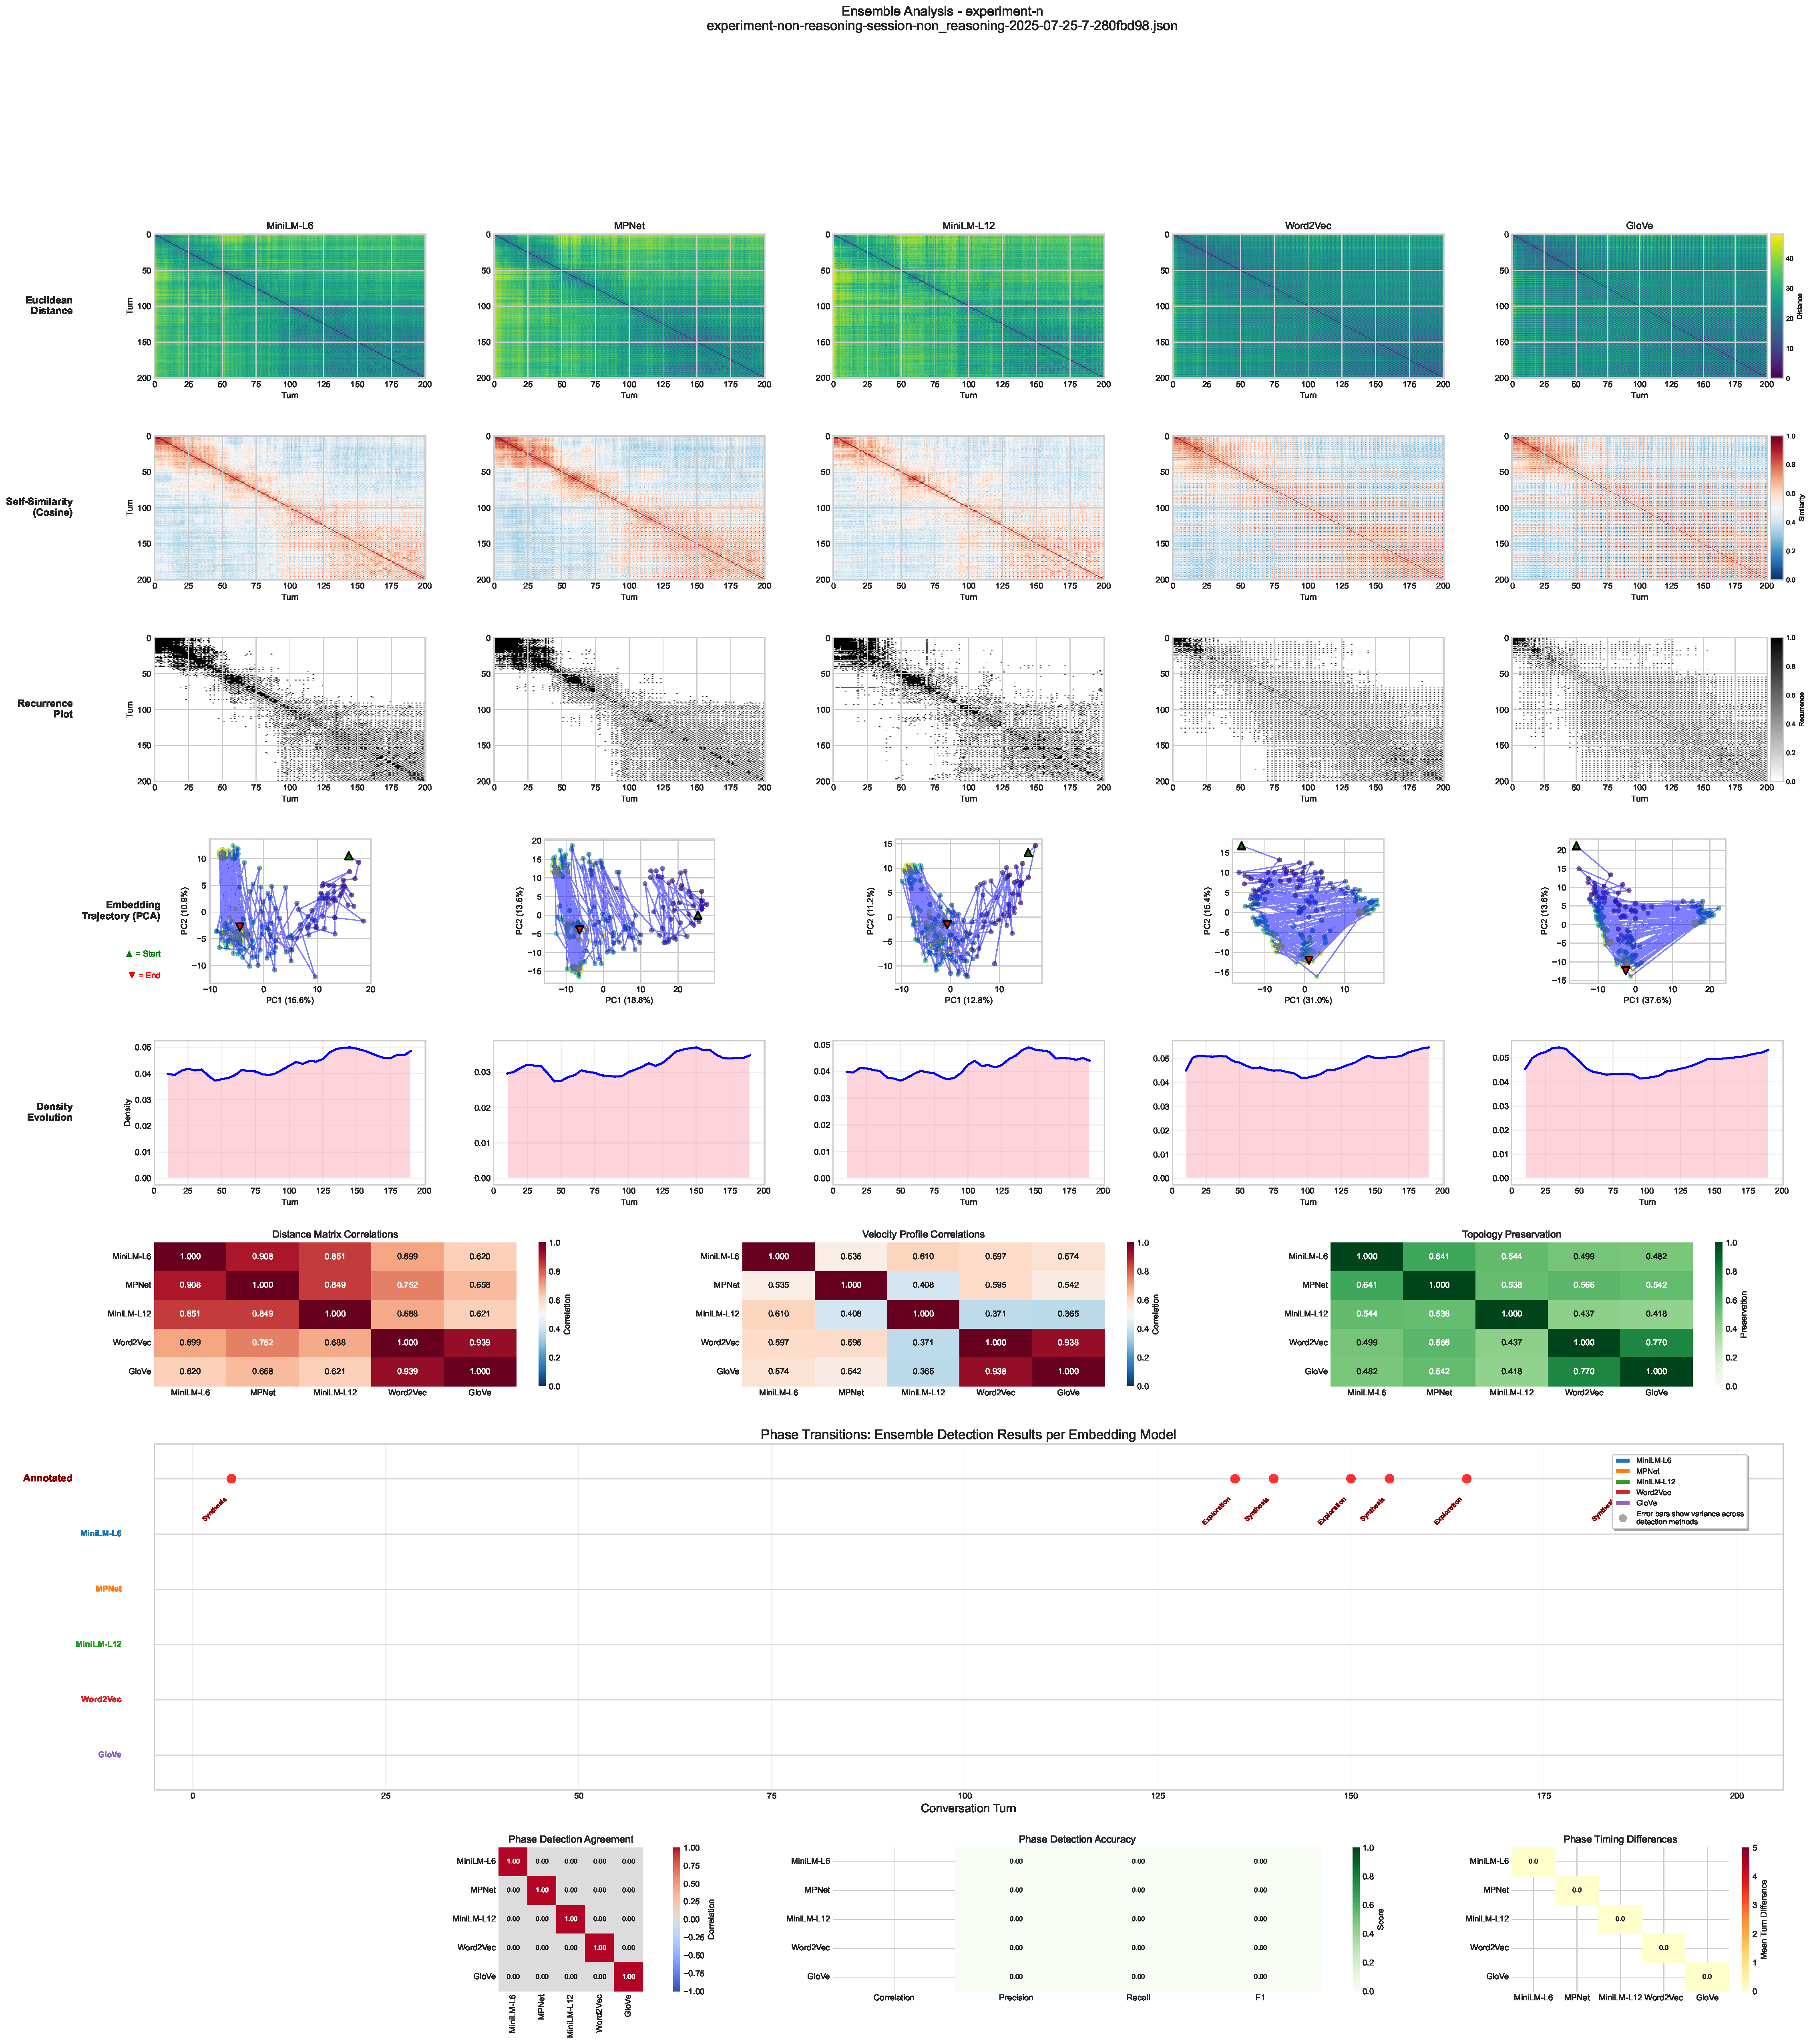
\includepdf[pages=1, pagecommand={\thispagestyle{plain}\label{fig:non_reasoning_2}}]{../analysis/analysis_output/figures/ensemble/pdf/experiment-non-reasoning-session-non_reasoning-2025-07-25-7-280fbd98_ensemble.pdf}
}

\end{document}